% !TEX encoding = UTF-8 Unicode
% Build with pdfLaTeX through build.sh; pnureport.cls is the unmodified PNU class.
\documentclass{pnureport}
\usepackage[T1]{fontenc}
\usepackage{booktabs,longtable,array,tabularx,amssymb}
\usepackage{graphicx,subcaption,placeins}
\usepackage[hidelinks]{hyperref}
\usepackage{tikz,pgfplots}
\usetikzlibrary{arrows.meta,positioning,calc,fit,shapes.geometric}
\pgfplotsset{compat=1.18}
\hypersetup{pdftitle={컴퓨터 비전과 역기구학 기반 SO-ARM101 로봇팔의 블록 이동 및 적재 시스템},pdfauthor={Sim2Real},pdfsubject={졸업과제 최종보고서}}
\renewcommand{\bibname}{참고 문헌}
\graphicspath{{figures/}}
\newcolumntype{L}[1]{>{\raggedright\arraybackslash}p{#1}}
\newcolumntype{Y}{>{\raggedright\arraybackslash}X}
\renewcommand{\arraystretch}{1.2}
\setlength{\tabcolsep}{5pt}
\setlength{\headheight}{16pt}
\setcounter{tocdepth}{2}
\setcounter{secnumdepth}{2}
\emergencystretch=2em
\raggedbottom
\reporttitle{컴퓨터 비전과 역기구학 기반\\SO-ARM101 로봇팔의\\블록 이동 및 적재 시스템}
\reportteam{Sim2Real}
\reportauthor{202170116 윤민석 0620yms@gmail.com\\202045106 김주환 kjhpooh386@naver.com\\202055575 이동근 ehdrms3835@gmail.com}
\reportadvisor{김종덕}
\reportdate{2026년 9월}
\begin{document}
\maketitle
\pagenumbering{roman}
\chapter*{초록}
\thispagestyle{plain}
본 과제는 SO-ARM101 로봇팔로 다섯 블록을 180초 이내 지정 영역으로 옮기고, 별도의 미션에서 블록을 적재한 뒤 5초간 유지하는 시스템을 목표로 하였다. 초기에는 ACT와 SmolVLA로 단일 블록 이동을 학습했으나, 시작 위치의 범위와 카메라 조건이 달라질 때 안정적인 수행을 확보하기 어려웠다. ACT와 컴퓨터 비전·역기구학(CV+IK)을 결합하는 시도에서도 파지 안정성과 시연 재수집 부담이 남아, CV+IK 기반 제어를 구현하고 실행 자료를 학습용으로 기록하도록 구성하였다.

최종 시스템은 색상·형상 기반 블록 검출, 평면 좌표 변환, IK 파지·배치 계획과 센서 기반 파지 확인을 유한상태기계로 연결하였다. 단계별 실패 분석으로 캘리브레이션, 파지 방향과 복구 동작을 보완한 뒤, 1차 미션은 30회 중 28회(93.3\%)에서 180초 내 다섯 블록 배치를 완료하였다. 재시도 포함 파지는 170회 중 148회(87.1\%) 성공했으며, 두 미션은 블록을 작업 반경 밖으로 밀어낸 뒤 시간 초과로 실패하였다. 최종 아홉 점 캘리브레이션의 적합 RMS는 5.15\,mm, 최대 leave-one-out(LOO) 오차는 13.53\,mm였다. 이는 영상 좌표와 기구학 모델 기준점 사이의 정합 오차이며, 실제 파지 정확도는 미션 수행 결과와 함께 평가하였다.

2차 미션은 5단 적재를 목표로 20회 시도하였다. 수행 도중 최대 높이 기준으로 3단에는 20회, 4단에는 17회 도달했으며 5단에는 도달하지 못했다. 재시도 포함 파지는 113회 중 94회(83.2\%) 성공하였다. 높이별 도달 횟수는 종료 시 높이나 해제 후 5초 유지 성공률을 뜻하지 않는다. 실행 자료를 자동 수집하는 Task3을 구현하여 첫 라운드에서 5개 에피소드, 2{,}111프레임을 186초에 저장하였다. 정책 재학습과 성능 비교는 수행하지 않았다.

\medskip
\noindent\textbf{주요어:} SO-ARM101, 모방학습, 컴퓨터 비전, 역기구학, 유한상태기계, 파지 검증

\clearpage
\tableofcontents
\clearpage
\pagenumbering{arabic}
\chapter{서론}
\section{연구 배경}
본 과제의 목표는 SO-ARM101 로봇팔로 다섯 블록을 제한시간 안에 지정 영역으로 옮기고, 후속 미션에서 적재하는 것이다. 이하에서는 SO-ARM101을 SO-101로 표기한다. 초기에는 이동형 로봇의 물체 수집을 검토했으나 과제 규격이 바뀌면서 SO-101 블록 조작으로 범위를 변경하였다. 개발 환경에서 개별 동작을 성공시키는 것과 함께, 장비를 실제 시연장으로 옮긴 뒤에도 여러 블록을 반복 처리할 수 있어야 했다.

초기에는 리더암으로 단일 블록을 집어 중앙 목표 지점으로 옮기는 동작을 시연하고, 이를 ACT와 SmolVLA로 학습하였다. 시작 위치를 한정하면 수행이 나아졌지만 작업 영역 전체로 범위를 넓혔을 때는 안정적인 동작을 얻기 어려웠다. ACT와 컴퓨터 비전·역기구학(CV+IK)을 결합한 방식에서도 카메라 위치 변화에 따른 성능 변동과 시연 재수집 부담이 남았다.

이에 크기와 색상이 정해진 블록과 고정 작업 평면의 조건을 활용해 CV+IK 기반 제어를 구성하였다. 검출 위치, 좌표 변환, 파지 확인과 재시도를 나누어 점검하면서 동작을 보완하였으며, 반복 실행을 학습 자료로 저장하여 수동 시연 수집의 부담도 줄이고자 하였다.

\section{초기 접근의 한계와 설계 요구}
첫째, 특정 시작 위치에서 얻은 결과를 작업 영역 전체의 수행으로 확장할 수 있어야 했다. 단일 블록이라도 위치와 접근 조건이 달라질 수 있으므로, 검출된 위치에서 실행 가능한 파지 자세를 생성해야 한다.

둘째, 환경 변화의 영향을 확인하고 조정할 수 있어야 했다. 카메라 고정·재캘리브레이션과 조명에 따른 검출 조정은 CV+IK에서도 필요하다. 검출 중심, 로봇 좌표, 목표 자세와 센서 판정을 각각 확인하여 수정할 단계를 좁히도록 하였다.

셋째, 개별 파지 실패를 전체 미션의 중단으로 이어지지 않게 해야 했다. 제한시간 내 여러 블록을 처리하려면 파지를 확인한 뒤 운반하고, 실패 시 재시도하거나 대상을 다시 선택해야 한다. 최종 제어 흐름은 이러한 판단과 복구 절차를 명시적으로 관리하도록 구성하였다.

\section{연구 목표}
\subsection{미션 규격과 성공 조건}
블록은 $40\times40\times20\,\mathrm{mm}$ 크기이며, 서로 다른 색의 블록 다섯 개를 사용한다. 미션 시작 시 각 블록은 넓은 면을 바닥에 둔 채 지정 영역 밖에 놓인다. 블록끼리 맞닿을 수는 있지만 위아래로 겹치지는 않는다. 두 미션은 블록을 다시 배치한 뒤 각각 수행한다. 목표와 평가 조건은 표~\ref{tab:mission}과 같다.

\begin{table}[htbp]
\centering
\caption{과제 미션의 목표와 평가 조건}\label{tab:mission}
\begin{tabularx}{\linewidth}{@{}L{0.16\linewidth}YY@{}}
\toprule
항목 & 1차 미션: 이동 & 2차 미션: 적재 \\
\midrule
목표 & 다섯 개 블록을 지정 영역에 배치 & 다섯 개 블록을 수직으로 적재 \\
제한시간 & 180초 & 300초 \\
지정 영역 & \multicolumn{2}{l}{$200\times100\,\mathrm{mm}$ 내부 영역} \\
인정 조건 & 경계 20\,mm 이내 걸침, 세로 세움과 일부 겹침 허용. 적재는 불인정 & 적재 상태를 5초 이상 안정적으로 유지 \\
부분 수행 & 시간 종료 시 영역에 놓인 블록 수 & 시간 종료 시 적재한 블록 수 \\
\bottomrule
\end{tabularx}
\end{table}

지정 영역은 로봇 베이스에서 약 25\,cm 떨어진 곳에 두며, 제어할 때는 네 꼭짓점을 로봇 베이스 좌표계에 등록한다.

신경망은 최대 하나까지 사용할 수 있으나 필수는 아니다. 최종 CV+IK 시스템은 신경망 없이 영상 처리와 기구학 계산으로 동작한다.

\subsection{세부 연구 목표}
영상에서 지정 영역 밖의 블록을 골라 로봇 좌표로 변환하고, 관절 한계와 그리퍼 방향을 고려한 접근·파지·이동 자세를 생성한다. 파지 확인과 재시도를 포함한 상태 흐름으로 블록을 반복 처리하며, 단계별 자료를 기록해 실패 지점을 추적한다. 적재 미션으로 동작을 확장하고, CV+IK의 실행 자료를 학습 데이터로 저장하여 향후 모방학습을 다시 시도할 기반을 마련한다.

본 연구는 기존 영상 처리와 기구학 도구를 과제 조건에 맞게 통합하고, 실패 복구와 실행 자료 수집까지 연결하는 데 초점을 두었다. 2장은 관련 기술, 3장은 설계와 구현, 4장은 실험 결과와 한계를 설명하며, 5장에서 결론과 후속 연구를 제시한다.
\FloatBarrier

\chapter{연구 배경}
\section{SO-101 플랫폼과 관측 장치}
SO-101은 리더암과 팔로워암을 이용한 텔레오퍼레이션 환경을 구성할 수 있는 로봇팔이다. LeRobot의 장비 문서는 조립, 통신, 캘리브레이션 및 리더·팔로워 구성 절차를 제공한다\cite{so101}. 본 과제는 리더암으로 시연과 캘리브레이션 자세를 만들고, 팔로워암으로 실제 블록 조작을 수행하였다. 팔의 위치·방향을 제어하는 다섯 관절과 그리퍼 개폐 축을 구분하여 다룬다.

초기 모방학습 단계에서는 손목 카메라와 상단 카메라를 사용하였다. 좌표 변환과 파지 계획은 고정된 상단 관측 카메라를 기준으로 하며, 최근에는 파지 검증을 보완하기 위해 손목 카메라를 다시 장착하는 작업을 진행하고 있다(3장). 비스듬한 시점에서 생기는 작업 평면의 원근 변형은 homography로 보정한다. 평면과 높이가 다른 물체에는 잔여 투영 오차가 발생하므로, 변환의 기준 높이를 블록 윗면에 맞추었다.

\begin{figure}[htbp]
\centering
\begin{subfigure}{0.61\linewidth}
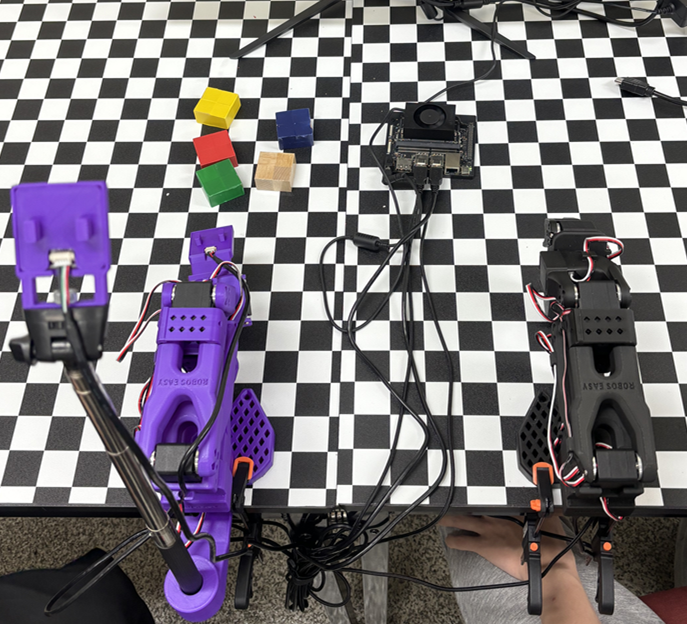
\includegraphics[width=\linewidth]{setup_early.png}
\caption{중간보고서 시점의 장비 배치}
\end{subfigure}\hfill
\begin{subfigure}{0.32\linewidth}
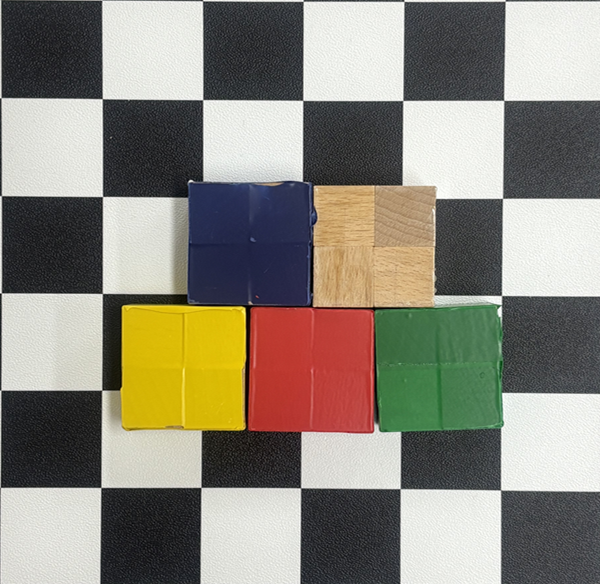
\includegraphics[width=\linewidth]{blocks.png}
\caption{과제 대상 블록}
\end{subfigure}
\caption{모방학습 단계의 장비 배치와 과제 대상 블록.}
\label{fig:hardware}
\end{figure}

팔로워의 관절 위치와 부하 정보는 제어와 결과 확인에 사용된다. 관절각의 피드백으로 동작 보간의 시작 자세를 정하고, 그리퍼의 위치와 부하로 빈손 닫힘과 물체를 물고 있는 상태를 구분한다. 그리퍼 위치는 장비 캘리브레이션에 따른 정규화 값이며, 부하는 힘 단위로 교정하지 않은 서보 피드백 값이다.

\section{고전 컴퓨터 비전 기반 블록 검출}
HSV 색 공간에서 OpenCV의 채널별 하한·상한 임계값으로 이진 마스크를 생성하여 블록 후보를 만든다\cite{opencv-hsv}. 빨강처럼 색상 범위의 양 끝에 걸리는 색은 두 구간의 마스크를 합쳐 처리한다. 색 임계값은 고정된 장면의 관측을 바탕으로 정한 설정이며, 조명과 배경이 달라지면 재검토가 필요하다.

색이 비슷한 배경을 배제하기 위해 윤곽선의 면적과 회전 사각형, 볼록 껍질을 함께 사용한다. 윤곽선 속성을 이용한 면적·종횡비·solidity 등의 계산은 OpenCV에서 제공하는 기본 연산으로 구성할 수 있다\cite{opencv-contour}. 윤곽선 면적을 $A$, 회전 경계 사각형의 폭과 높이를 $w,h$, 볼록 껍질의 면적을 $A_{\mathrm{hull}}$이라 하면 다음과 같이 정의한다.
\begin{equation}
 r=\frac{\max(w,h)}{\min(w,h)},\qquad
 f=\frac{A}{wh},\qquad
 s=\frac{A}{A_{\mathrm{hull}}}.
\end{equation}
여기서 $r$은 종횡비, $f$는 채움 비율, $s$는 solidity이다. 긴 테이프 조각은 종횡비가 커질 수 있고, 내부가 빈 경계 형태는 채움 비율이 낮아질 수 있다. 실제 블록도 그림자나 측면의 영향으로 이상적인 정사각형과 다르게 검출되므로, 형상 조건은 실환경 결과와 함께 조정해야 한다.

색상과 형상은 후보 생성의 기준이고, 실제 제어 대상의 결정에는 작업 범위와 배치 상태도 필요하다. 본 과제에서 사용한 색 기준점 할당, 형상 임계값과 영역 필터의 적용 순서는 3장에서 설명한다.

\section{평면 좌표 변환과 캘리브레이션}
\subsection{Homography의 적용 범위}
Homography는 두 평면 좌표 표현 사이의 사영 변환을 나타내며, 평면의 원근 변형을 보정하거나 대응점 관계를 표현하는 데 사용된다\cite{opencv-homography}. 본 시스템은 영상 픽셀 $(u,v)$와 로봇 베이스 프레임의 평면 좌표 $(x,y)$를 다음과 같이 연결한다.
\begin{equation}
 \lambda\begin{bmatrix}x\\y\\1\end{bmatrix}
 =H\begin{bmatrix}u\\v\\1\end{bmatrix},\quad
 x=\frac{h_{11}u+h_{12}v+h_{13}}{h_{31}u+h_{32}v+h_{33}},\quad
 y=\frac{h_{21}u+h_{22}v+h_{23}}{h_{31}u+h_{32}v+h_{33}}.
\end{equation}
실제 계산에서는 분모로 정규화한 좌표를 사용한다. 로봇 베이스를 원점으로 정의하여 검출 위치, 지정 영역과 거리 기반 대상 선택을 같은 좌표계에서 표현한다. 체스판은 대응점 수집과 카메라 드리프트 관찰에 사용한다.

카메라 마운트가 움직이거나 기준 높이가 바뀌면 픽셀과 로봇 좌표의 대응 관계도 달라져 재캘리브레이션이 필요하다.

\subsection{잔차와 일반화 오차}
캘리브레이션의 적합 잔차는 대응점 $\boldsymbol{p}_i$와 변환으로 예측한 위치 $\hat{\boldsymbol{p}}_i$의 차이로 계산한다. $N$개 점에 대한 제곱평균제곱근 오차는 다음과 같다.
\begin{equation}
 e_i=\|\hat{\boldsymbol{p}}_i-\boldsymbol{p}_i\|_2,\qquad
 \mathrm{RMS}=\sqrt{\frac{1}{N}\sum_{i=1}^{N} e_i^2}.
\end{equation}
같은 점으로 변환을 적합하고 평가한 잔차는 새로운 위치의 오차를 직접 나타내지 않는다. 이에 따라 한 점을 제외하고 나머지 점으로 변환을 적합한 뒤 제외한 점을 평가하는 leave-one-out(LOO) 결과를 함께 확인한다. 또한 대응점의 로봇 좌표 자체를 FK로 기록하므로, 이 평가에는 카메라뿐 아니라 자세 기록과 기구학 기준의 오차가 함께 포함될 수 있다.

\section{역기구학과 상태 기반 제어}
\subsection{목표 위치에서 관절 자세로의 변환}
역기구학은 목표 자세 $T_d$를 만족하는 관절값 $\boldsymbol{q}$를 구하는 문제이며, 수치해법에서는 초기값과 도달 가능성이 수렴 결과에 영향을 미친다\cite{modern-robotics}. 본 구현은 URDF 모델과 PlaCo의 운동학 풀이 기능을 사용한다. PlaCo는 관절 제한 등을 포함한 작업 공간의 역기구학 문제를 구성할 수 있다\cite{placo}.

SO-101에서는 위치와 모든 방향을 임의로 독립 지정할 수 없으므로, 목표 위치뿐 아니라 접근 방향과 관절 한계를 함께 검사해야 한다.

역기구학은 접근·파지·운반 등 소수의 웨이포인트에서 수행하며, 세부 보간 방식과 실행 결과 확인은 3장에서 설명한다.

\subsection{유한상태기계와 파지 확인}
유한상태기계(FSM)는 대상 선택부터 배치까지의 단계를 상태로 분리하여 실행 조건과 실패 경로를 명시한다. 파지가 확인되지 않으면 운반 단계로 넘어가지 않는 조건이 핵심이며, 세부 흐름은 3장에서 설명한다.

조작 결과를 평가할 때는 파지 확인, 운반 중 물체 유지, 배치 후 안착, 적재 후 유지를 구분해야 한다. 현재 센서 판정은 그리퍼가 물체를 물고 있는지를 확인하며, 이후의 안착과 적재 유지까지 자동으로 보장하지는 않는다. 이 구분은 실패 분석과 학습 데이터의 성공 라벨을 정의할 때에도 적용된다.

\FloatBarrier

\chapter{연구 내용}
\section{모방학습 실험과 CV+IK 전환}
\subsection{단일 블록 시연의 범위 축소와 재확장}
초기에는 리더암의 시연으로 블록 조작 동작을 학습하도록 설계하였다. ACT(Action Chunking with Transformers)는 연속된 여러 시점의 행동을 묶어 예측하는 모방학습 방법이며\cite{act}, SmolVLA는 영상·언어 입력을 행동 생성에 연결하는 모델이다\cite{smolvla}. LeRobot으로 시연 수집과 학습·추론 환경을 구성하고, 로봇 제어기와 정책 서버는 gRPC 원격 추론으로 연결하였다.

첫 실험은 작업 영역 전체에 단일 블록을 무작위로 놓고, 이를 텔레오퍼레이션으로 집어 중앙 목표 지점에 옮기는 것이었다. 약 100개 에피소드를 수집하여 ACT와 SmolVLA를 학습·실행했으나, 팀이 관찰한 수행 성공률은 약 2--10\%로 낮았다. 따라서 처음부터 넓은 시작 위치를 다루기보다 한정된 조건에서 동작을 학습할 수 있는지 먼저 확인하였다.

두 번째 단계에서는 특정 시작 위치에서 목표 지점까지 옮기는 시연을 중심으로 51개 에피소드를 수집하였다. 이 조건에서 단일 블록 이동은 50회 중 29회(58\%) 성공하였다. 위치를 한정하면 수행이 나아지는 것을 보고 시작 위치를 다시 전 영역으로 넓혔으며, 약 120개 에피소드로 ACT와 SmolVLA를 학습하였다. 그러나 이때의 수행 성공률은 약 10--20\%로 다시 낮아졌다. 세 단계 모두 블록 하나를 집어 옮기는 과제로, 블록 수를 늘리지 않고 시작 위치의 범위를 바꾸었다.

\begin{table}[htbp]
\centering
\caption{초기 단일 블록 모방학습의 조건과 수행 결과}\label{tab:early}
\begin{tabularx}{\linewidth}{@{}L{0.14\linewidth}YL{0.17\linewidth}L{0.23\linewidth}@{}}
\toprule 단계 & 블록의 시작 조건 & 시연 에피소드 & 수행 성공 \\
\midrule
전 영역 수집 & 단일 블록, 전 영역 무작위 위치 & 약 100개 & 약 2--10\% \\
범위 축소 & 단일 블록, 특정 시작 위치 중심 & 51개 & 29/50회 (58\%) \\
범위 재확장 & 단일 블록, 전 영역 무작위 위치 & 약 120개 & 약 10--20\% \\
\bottomrule
\end{tabularx}
\end{table}

표~\ref{tab:early}의 51개 시연과 29/50회는 실험 집계값이며, 나머지 수집량과 성공률 범위는 팀의 회고에 따른 근사치이다. 단계별 작업 범위와 학습 조건이 달라 데이터 수 증가만의 효과로 해석하지 않았으며, 모델별 세부 성공률을 구분할 기록도 확보하지 못하였다.

\subsection{ACT와 CV+IK의 하이브리드 시도}
단일 블록의 파지와 이동에서도 성공이 불안정하자, 학습 정책이 전체 동작을 담당하는 부담을 줄이기 위해 ACT와 CV+IK의 하이브리드 방식을 시도하였다. 파지에는 ACT를 사용하고 배치는 IK로 연결하는 역할 분담을 검토·시험하였다. SmolVLA 대신 ACT를 선택한 이유는 팀의 비교 실험에서 추론이 더 빠르고 수행 성공률도 일관되게 높았기 때문이다. 이는 당시 장비와 학습 조건에서의 관찰이며, 모델별 지연시간과 성공률을 같은 조건에서 측정한 비교표는 확보하지 못하였다.

ACT의 학습·추론 설정을 조정했지만 약 60\%를 넘는 안정적인 수행으로 끌어올리기 어려웠다. 팔이 목표 근처에 도달한 뒤에도 블록을 잡지 못하는 경우에는 영상 입력, 정책 출력과 실제 접촉 중 어느 부분을 바꿔야 할지 판단하기 어려웠다. 하이브리드로 정책의 역할을 줄여도 파지의 불안정성이 남으면 반복 미션 전체를 안정화하기 어려웠다.

\subsection{CV+IK 기반 제어로의 전환}
카메라를 조금 옮긴 뒤 기존 정책의 수행이 달라져 시연부터 다시 수집해야 했으며, 100개 이상의 에피소드를 사람이 다시 녹화하는 부담이 컸다. 장비를 시연장으로 옮긴 뒤에도 같은 수집·학습·평가 과정을 반복해야 할 수 있어 현장에서 조정할 수 있는 제어 방식이 필요하였다.

이에 크기와 색상이 정해진 블록과 고정 작업 평면에 맞추어 CV+IK 제어를 구현하였다. 반복적인 수동 시연을 줄이기 위해 실행 과정도 학습용으로 기록하고자 하였으며, 동작을 보완한 뒤 이를 Task3의 자동 수집 기능으로 구현하였다. 저장한 자료를 이용한 정책 재학습은 후속 과제로 남았다.

CV는 블록 중심과 방향을, 캘리브레이션은 로봇 좌표를, IK는 후보 자세와 도달성을 제공한다. 그리퍼 위치·부하는 파지 여부를 확인하고 FSM은 재시도와 대상 전환을 관리한다. 중간 결과를 분리하면 검출 실패, 좌표 편차, 계획 불가와 빈손 파지를 각각 점검할 수 있다. 기존 모터 통신과 장비 제어 경험은 이 경로에 재사용하였다.

\begin{table}[htbp]
\centering
\caption{초기 실험에서 관찰한 제약과 전환 후의 설계 대응}
\begin{tabularx}{\linewidth}{@{}YY@{}}
\toprule 초기 운용에서의 제약 & CV+IK의 대응 \\
\midrule
시작 위치 확대 후 단일 블록 수행 불안정 & 검출 위치를 로봇 좌표로 변환하고 후보별 IK 도달성 확인 \\
카메라 변경 후 반복 시연 수집 부담 & 카메라 재고정·재캘리브레이션 후 실행 자료를 Task3으로 기록 \\
실패 원인의 분리 어려움 & 검출·좌표·IK·센서·상태 전이의 중간 결과 기록 \\
하이브리드에서도 남은 파지 실패 & 센서 파지 확인 뒤 운반, 회전 재시도와 대상 재선택 \\
\bottomrule
\end{tabularx}
\end{table}

CV+IK에서도 카메라 고정과 마운트 변경 후 재캘리브레이션, 조명에 따른 검출 조정이 필요하다. 환경 변화의 영향을 없앤다는 가정 대신, 관측과 제어를 점검·보정하고 실행 자료를 다시 수집할 수 있는 구조를 선택하였다. 두 방법의 일반화 성능을 동일 조건에서 비교하는 실험은 수행하지 않았다.
\FloatBarrier

\section{최종 시스템 아키텍처}
\subsection{구성 요소와 관측 경로}
\label{sec:system-config}
기본 제어는 고정 상단 카메라의 블록 검출, 평면 좌표 변환과 IK, 그리퍼 위치·부하 판정으로 구성된다. 미션 평가에는 ArUco 위치 추정과 손목 카메라 색상 게이트를 추가 관측 기능으로 사용하였다. 이하에서는 기본 제어 구조와 추가 관측 기능의 역할을 구분하여 설명한다.

시스템은 카메라 서비스, 인식 모듈, 기구학·동작 모듈, 상태 제어기와 로봇 입출력으로 구성된다. 카메라 서비스가 USB 장치를 단독으로 읽어 최신 프레임을 제공하고, 미션 실행기는 HTTP로 받은 최신 정지 영상(snapshot)에서 제어할 블록을 검출한다. 브라우저 관제 화면에는 MJPEG 영상과 분석 결과를 표시한다. 화면에 겹쳐 그린 좌표는 운영자의 점검용이며 파지 계획의 입력으로 사용하지 않는다.

\begin{figure}[htbp]
\centering
\begin{tikzpicture}[node distance=9mm,
box/.style={draw,rounded corners,align=center,text width=5.4cm,minimum height=9mm,font=\small},
arr/.style={-{Latex},thick}]
\node[box] (cam) {고정 카메라 / 카메라 서비스};
\node[box,below=of cam] (cv) {최신 snapshot / 고전 CV\\영역 밖 블록 중심·방향·색};
\node[box,below=of cv] (ik) {베이스 좌표 / 파지 후보 생성\\IK 도달성 검사와 웨이포인트};
\node[box,below=of ik] (fsm) {FSM / 관절 궤적 실행\\파지 확인·운반·배치·재시도};
\node[box,below=of fsm] (robot) {SO-101 팔로워\\관절 위치·그리퍼 부하};
\node[box,text width=3.4cm,right=13mm of cv] (ui) {브라우저 관제\\MJPEG·검출·FK 표시};
\draw[arr] (cam)--(cv);
\draw[arr] (cv)--(ik);
\draw[arr] (ik)--(fsm);
\draw[arr] (fsm)--(robot);
\draw[arr] (cam.east)-|(ui.north);
\draw[arr,dashed] (robot.west)--++(-9mm,0)|-node[pos=0.75,left,font=\scriptsize]{측정 피드백}(fsm.west);
\draw[arr,dashed] (robot.east)-|(ui.south);
\end{tikzpicture}
\caption{기본 CV+IK 제어 경로와 관제 구성. 실선은 주 입력·실행 경로, 점선은 측정 상태의 전달이다. 추가 관측 기능은 절~\ref{sec:additional-observation}에서 설명한다.}
\label{fig:architecture}
\end{figure}

\FloatBarrier
\subsection{전체 상태 흐름과 판단 조건}
제어 상태는 SELECT, PICK, VERIFY, TRANSPORT, PLACE 순으로 이어진다. SELECT는 카메라 시야를 확보하는 대기 자세(HOME)에서 최신 영상을 받아 블록을 고른다. PICK은 도달 가능한 파지 후보를 실행하고 센서값을 확인한다. PICK이 통과해도 VERIFY에서 파지 상태를 다시 검사하며, 물체가 확인된 경우에만 TRANSPORT로 넘어간다. 실패하면 후보를 바꾸거나 SELECT로 돌아간다(그림~\ref{fig:fsm}).

\begin{figure}[htbp]
\centering
\begin{tikzpicture}[
state/.style={draw,rounded corners,text width=3.1cm,minimum height=10mm,align=center,font=\small},
decision/.style={draw,diamond,aspect=2.5,text width=2.1cm,align=center,inner sep=1pt,font=\small},
arr/.style={-{Latex},thick}]
\node[state] (sel) at (0,0) {SELECT\\관측과 대상 선택};
\node[state] (pick) at (0,-1.7) {PICK\\후보별 파지 시도};
\node[decision] (ver) at (0,-3.4) {VERIFY\\파지 확인?};
\node[state] (tr) at (0,-5.1) {TRANSPORT\\슬롯 상공 이동};
\node[state] (pl) at (0,-6.5) {PLACE\\블록 해제};
\node[state,text width=2.5cm] (retry) at (-4.3,-3.4) {재시도 / 순회 보류\\시도 이력 관리};
\node[state,text width=2.7cm] (done) at (5.4,0) {DONE\\관측 기반 완료};
\draw[arr] (sel)--node[right,font=\scriptsize]{대상 있음}(pick);
\draw[arr] (pick)--(ver);
\draw[arr] (ver)--node[right,font=\scriptsize]{예}(tr);
\draw[arr] (tr)--(pl);
\draw[arr] (ver.west)--node[above,font=\scriptsize]{아니오}(retry.east);
\draw[arr] (pick.west)-|node[pos=0.25,above,font=\scriptsize]{PICK 실패}(retry.north);
\draw[arr] (retry.west)--++(-5mm,0)|-(sel.west);
\draw[arr] (pl.east)--++(8mm,0)|-(sel.south east);
\draw[arr] (sel)--node[above,align=center,font=\scriptsize]{영역 밖 검출\\연속 5초 부재}(done);
\draw[arr] (sel.north east)--++(0,6mm)-|(sel.north west);
\node[font=\scriptsize,anchor=south] at (0,1.15) {대상 미확정 / 새 프레임 재관측};
\end{tikzpicture}
\caption{1차 미션의 상태 흐름과 성공/실패 분기. 완료 판정에는 유효한 새 프레임만 사용한다. 외부 시간 제한에 의한 중단은 완료와 구분한다.}
\label{fig:fsm}
\end{figure}

\FloatBarrier

\subsection{외부 기술과 팀의 구현 범위}
\begin{table}[htbp]
\centering
\caption{외부 기술의 활용과 팀의 설계 및 구현}
\begin{tabularx}{\linewidth}{@{}L{0.16\linewidth}L{0.29\linewidth}Y@{}}
\toprule
구성 & 활용한 기반 기능 & 팀의 설계 및 구현 \\
\midrule
인식 & OpenCV 색 변환, 윤곽선과 평면 변환 & 미터법 형상 필터, 색 기준점 할당, 영역 밖 대상 선택 \\
기구학 & PlaCo의 URDF 기반 FK/IK 풀이 & 시드와 중립 손목 방향, 후보 보정, 접근 높이 탐색 \\
장비 제어 & LeRobot 장비 통신과 관절 명령 제한 & 입출력 추상화, 측정 자세 기반 보간, 파지 판정 연결 \\
미션 실행 & Python 상태 및 자료 구조 & FSM, 후보 재시도와 순회 보류, 동적 슬롯, 적재 PLACE 전략 \\
관제·기록 & 영상 입출력과 HTTP 기본 기능 & 카메라 단독 소유, 최신 프레임 전달, FK 표시, 실험 이력 관리 \\
\bottomrule
\end{tabularx}
\end{table}

카메라 장치의 접근 충돌을 막기 위해 영상 획득을 별도 서비스로 분리하였다. 관제 화면의 FK 표시는 제어기가 공유한 관절 측정값을 사용하며, 영상 위에 검출 후보와 FK 투영 위치를 함께 표시한다.

\section{블록 검출과 대상 선택}
\subsection{미터법 영상과 후보 생성}
지정 영역의 빨간 테이프가 빨간 블록과 함께 검출되는 문제가 있었다. 색 임계값만 사용하면 같은 색의 경계가 후보에 남는다. 블록의 채워진 정사각형 윤곽과 길쭉하거나 내부가 빈 테이프 윤곽을 구분하도록 형상 필터를 추가하였다. 색상으로 후보를 찾은 뒤 기하 특성으로 거르는 방식이다.

입력 영상은 캘리브레이션 결과에 따라 로봇 평면 좌표에 대응하는 1\,mm/pixel 정사영 영상으로 변환한다. HSV 색 공간에서 색별 마스크를 만든 뒤 타원형 커널로 열림·닫힘 연산을 적용한다. 외부 윤곽선에서 면적, 회전 사각형과 형상 지표를 계산하므로 물체 크기 조건을 밀리미터 단위로 지정할 수 있다.

검출기의 주요 설정값은 표~\ref{tab:detector-config}와 같다. 단일 블록의 이상적인 상면 면적은 $40\times40=1,600\,\mathrm{mm}^2$이며, 측면·그림자·마스크 손실을 고려하여 후보 면적 범위에 여유를 두었다.

\begin{table}[htbp]
\centering
\caption{검출기의 설정값과 역할}\label{tab:detector-config}
\begin{tabularx}{\linewidth}{@{}L{0.31\linewidth}L{0.19\linewidth}Y@{}}
\toprule
항목 & 설정값 & 적용 목적 \\
\midrule
정사영 해상도 & 1\,mm/pixel & 형상 조건을 미터법으로 표현 \\
후보 면적 & 900--3,200\,$\mathrm{mm}^2$ & 작은 잡음·큰 배경 영역 배제 \\
최대 종횡비 & 1.6 & 길쭉한 테이프 후보 배제 \\
최소 채움 비율 & 0.65 & 비어 있는 경계 형태 배제 \\
최소 볼록도 & 0.78 & 지나치게 오목한 형상 배제 \\
형태학적 커널 & $9\times9$ pixel & 마스크 잡음과 윤곽 변동 완화 \\
중복 후보 거리 & 30\,mm 미만 & 겹친 색 마스크의 동일 물체 병합 \\
색상별 최대 후보 & 1개 & 과제의 색상별 단일 블록 조건 반영 \\
관측 부채꼴 & 반경 320\,mm, $-90^\circ$--$90^\circ$ & 제어 대상 관측 범위 제한 \\
\bottomrule
\end{tabularx}
\end{table}

후보는 면적, 종횡비와 채움 비율로 판별한다. 맞닿은 블록의 윤곽이 합쳐지거나 팔에 가려져 면적이 줄면 실제 블록도 제외될 수 있다. 이를 줄이기 위해 SELECT에서는 HOME으로 돌아가 시야를 확보하고 매 사이클 새 영상을 검출한다. 형상 필터 적용 전후의 검출 정확도는 따로 측정하지 않았다.

\subsection{색 기준점 할당과 영역 필터}
후보의 대표 색상·채도를 $(H,S)$, 기준점을 $(H_c,S_c)$라고 하면 구현의 거리 함수는 다음과 같다.
\begin{equation}
\Delta H=\min(|H-H_c|,180-|H-H_c|),\qquad
d=\sqrt{\left(\frac{2\Delta H}{128}\right)^2+
\left(\frac{S-S_c}{128}\right)^2}.
\end{equation}
색상은 원형 범위로 처리하고, 한 색에 기준점이 여러 개 있으면 가장 가까운 거리를 사용한다. 전체 후보--색 쌍을 거리순으로 정렬한 후 이미 할당한 후보나 사용한 색을 제외하면서 탐욕적으로 할당한다. 거리가 0.35를 넘는 후보는 미할당 상태로 남긴다.

동일한 블록이 여러 색 마스크에 잡힌 경우에는 채움 비율과 볼록도의 곱이 높은 후보를 우선하여 가까운 후보를 병합한다. 지정 영역 내부 후보는 블록 중심 좌표로 판정하여 색 할당 전에 제외한다. 이 순서를 통해 이미 배치한 블록이 색 할당을 차지하여 영역 밖의 후보를 가리는 상황을 줄였다.

1차 미션은 현재 검출된 후보 가운데 베이스 원점에서 가까운 블록을 먼저 선택한다. 색상별 블록이 하나씩이라는 조건을 이용하여 색 이름을 재시도 식별자와 슬롯 예약의 키로 사용한다. 동일한 색이 여러 개 존재하는 일반 작업으로 확장하려면 별도의 물체 추적 식별자가 필요하다.

\section{캘리브레이션과 좌표 관리}
\subsection{대응점 수집 절차}
영상의 블록 중심과 실제 그리퍼 접근 위치가 어긋나지 않도록 대응점 수집 조건을 정하였다. 블록 윗면과 빈 테이블은 높이가 다르며, 같은 위치에서 턱이 닿아도 손목 회전에 따라 FK 기준점 좌표가 달라질 수 있다. 대응점 수뿐 아니라 기준 평면과 손목 자세, 기록 항목을 함께 관리하였다.

대응점 하나를 기록할 때 같은 블록 위치에서 두 장면을 촬영하였다. 먼저 그리퍼 기준점을 블록 윗면 중앙에 맞추고 관절값과 접촉 자세 영상을 저장한다. 블록을 그대로 둔 채 팔을 물린 뒤 윗면이 드러난 영상에서 픽셀 중심을 찾는다. 첫 장면의 관절값으로 구한 FK 좌표와 두 번째 장면의 영상 좌표를 같은 점으로 연결한다. 그림~\ref{fig:calibration-pair}는 초기 수집 자료의 대응점 P4로 절차를 보여준다. 최종 보정에 사용한 대응점은 카메라 재고정 후 별도로 수집하였다.

\begin{figure}[!htbp]
\centering
\begin{subfigure}[t]{0.48\linewidth}
\centering
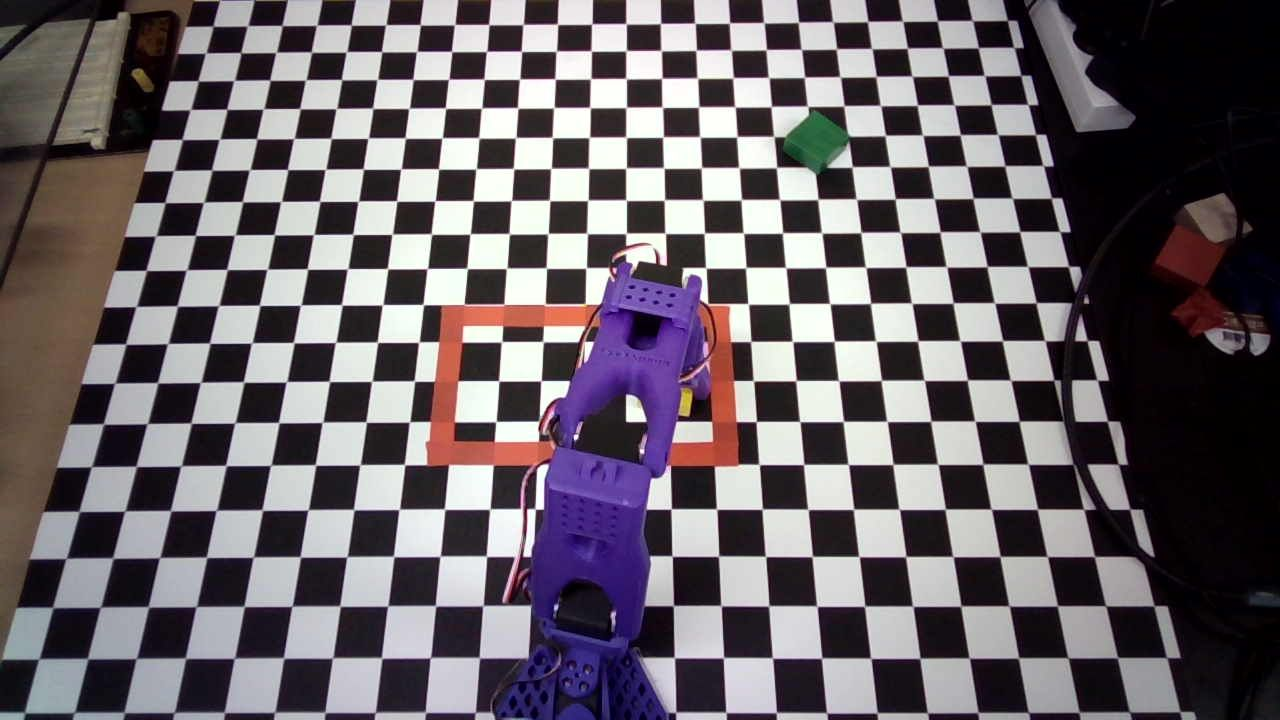
\includegraphics[width=\linewidth,trim=400bp 200bp 480bp 220bp,clip]{calibration_p4_contact.jpg}
\caption{접촉 자세에서 관절값 기록}
\small FK $(x,y)=(234.237,-43.885)$\,mm
\end{subfigure}\hfill
\begin{subfigure}[t]{0.48\linewidth}
\centering
\begin{tikzpicture}
\node[anchor=south west,inner sep=0] (photo) at (0,0) {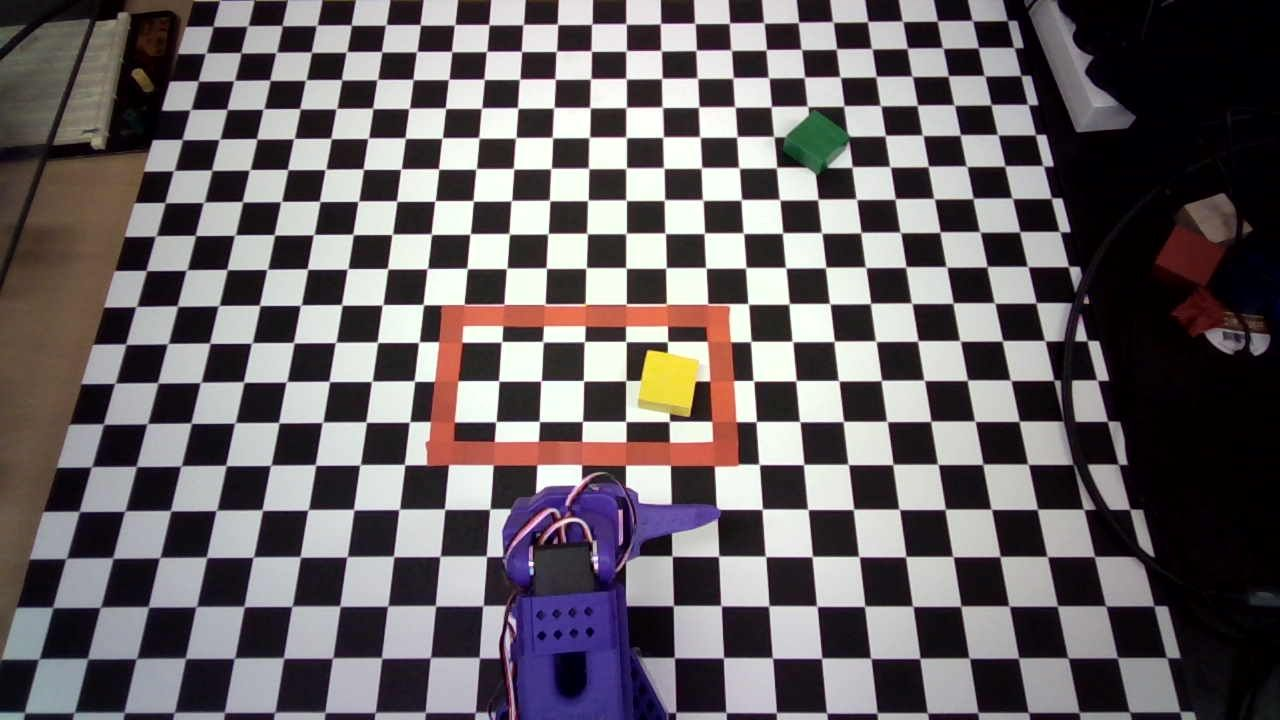
\includegraphics[width=\linewidth,trim=400bp 200bp 480bp 220bp,clip]{calibration_p4_clear.jpg}};
\begin{scope}[x={(photo.south east)},y={(photo.north west)}]
\draw[cyan!80!blue,line width=0.9pt] (0.66954,0.46207) circle[radius=2mm];
\draw[cyan!80!blue,line width=0.9pt] (0.645,0.46207)--(0.695,0.46207) (0.66954,0.43)--(0.66954,0.495);
\end{scope}
\end{tikzpicture}
\caption{팔을 물린 뒤 픽셀 중심 확인}
\small $(u,v)=(667.817,381.379)$\,pixel
\end{subfigure}
\caption{대응점 수집 절차의 예. 접촉 자세의 관절값으로 FK 좌표를 구하고, 팔을 물린 영상에서 같은 블록의 픽셀 중심을 기록한다. 두 사진은 원본의 같은 범위를 확대한 것이다.}
\label{fig:calibration-pair}
\end{figure}

수집 도구는 점 이름, 사진, 픽셀 좌표, FK 좌표와 관절값을 함께 저장하며 중단된 지점부터 수집을 재개할 수 있다. 베이스 좌표는 밀리미터로 관리하고 IK 라이브러리 경계에서 단위를 변환한다. 카메라 웹 뷰어의 검출 후보와 FK 투영점은 대응 관계를 점검하는 표시일 뿐, 실제 턱 위치로 사용하지 않는다.

손목 회전은 중립 근처로 유지한다. 같은 턱 접촉 상태라도 회전축과 URDF 그리퍼 기준점의 위치 관계 때문에 기록되는 FK 좌표가 바뀔 수 있기 때문이다. 따라서 좌표값만 남기는 대신 관절각을 보관하고, 캘리브레이션 자세와 런타임 파지 자세의 차이를 줄이는 절차를 사용하였다. 카메라를 다시 고정한 경우에는 대응점을 다시 수집하여 변경된 카메라 배치에 맞는 변환을 적용하였다.

\subsection{좌표 품질과 카메라 안정성 평가}
좌표 변환은 적합 RMS와 최대 LOO 오차로 평가하였다. 카메라 배치나 수집 자세가 바뀔 때 대응점을 재수집하였으며, 최종 평가에는 아홉 점으로 적합한 변환을 사용하였다. 좌표 정합 결과는 절~\ref{sec:calibration-results}에 제시하며, 실제 파지 여부는 그리퍼 센서와 미션 수행 결과로 확인하였다.

카메라 안정성은 기준 영상에 대한 대응 코너의 이동량으로 점검한다. 일부 코너의 검출 변동에 민감한 최댓값 대신 전체 변위 분포의 p95를 사용하였다. 카메라 고정 상태가 달라지면 기존 좌표 변환의 적용 여부도 다시 확인해야 한다.
\FloatBarrier
\section{역기구학과 궤적 실행}

\subsection{손목 과열에 대응한 중립 방향 선택}
초기에는 그리퍼 yaw를 베이스 기준으로 고정하였다. 팔이 선회할수록 손목이 반대로 비틀렸고, 결국 손목 서보가 과열 보호로 정지하였다. 이후에는 작업 위치별 중립 손목 방향을 기준으로 블록 면을 정렬하여 파지 방향을 유지하면서 손목 회전을 줄였다.

파지 계획은 선택한 블록의 좌표와 방향, 캘리브레이션의 파지 높이를 입력으로 받는다. URDF에 정의된 그리퍼 기준 좌표계를 목표 프레임으로 사용하고 접근축이 아래를 향하는 자세를 우선한다. 위치마다 가능한 관절 조합이 다르므로, FK로 구성한 자세 시드를 사용하고 어깨 선회각에 여러 오프셋 후보를 적용하여 해를 찾는다. 선회각의 오프셋 후보는 $0^\circ,\pm6^\circ,\pm12^\circ$이다.

블록 방향을 지정하지 않은 IK는 해당 위치의 중립 손목 방향을 기준으로 한다. 블록 면에 맞춰 잡을 때는 검출 윤곽의 최소 면적 회전 사각형에서 블록 방향 $\theta_b$를 구한다. 최종 파지 방향은 베이스 중심 작업 영역의 접선 방향 $\theta_t=\operatorname{atan2}(y,x)+90^\circ$에 가장 가까운 정사각형의 대칭 방향으로 정한다.
\begin{equation}
 \theta^*=\arg\min_{\theta\in\{\theta_b+k\cdot90^\circ\mid k\in\mathbb{Z}\}}
 \big|\operatorname{wrap}_{[-180^\circ,180^\circ)}(\theta-\theta_t)\big|.
\end{equation}
이 선택은 작업 영역의 접선과 블록 면을 함께 고려한다. 손목 회전의 안전성을 위해 실제 IK 해의 도달성도 확인하며, 과열 대응 전후의 온도 상승량과 연속 운용 시간은 별도로 비교하지 않았다.

\subsection{위치 보정에서 회전 재시도로의 변경}
초기에는 좌표 편차를 흡수하려고 반경·접선 방향의 경험적 보정과 네 위치 후보 $(0,15)$, $(-15,0)$, $(0,-15)$, $(15,0)$\,mm를 사용하였다. 후보 변경과 대상 재선택으로 동작을 이어 갔으나, 빈손 파지가 반복되거나 한 블록에 긴 시간이 소요되어 캘리브레이션과 파지 방향을 함께 점검하였다.

최종 기본 설정은 반경·전방 및 근거리 추가 보정을 0\,mm로 두고, 그리퍼 로컬 접선 방향의 5\,mm 보정을 사용한다. 위치 재시도 목록은 비워 두었다. 최초 실패나 하강 중단 뒤에는 같은 XY에서 파지 방향을 90도 회전한 후보를 한 번 시도한다. 두 회전 부호의 IK 해 가운데 도달 가능성과 손목 중립에 대한 편차를 고려해 하나를 선택한다. 회전 후보도 실패하면 재선택 또는 순회 보류로 이어진다.

\begin{figure}[htbp]
\centering
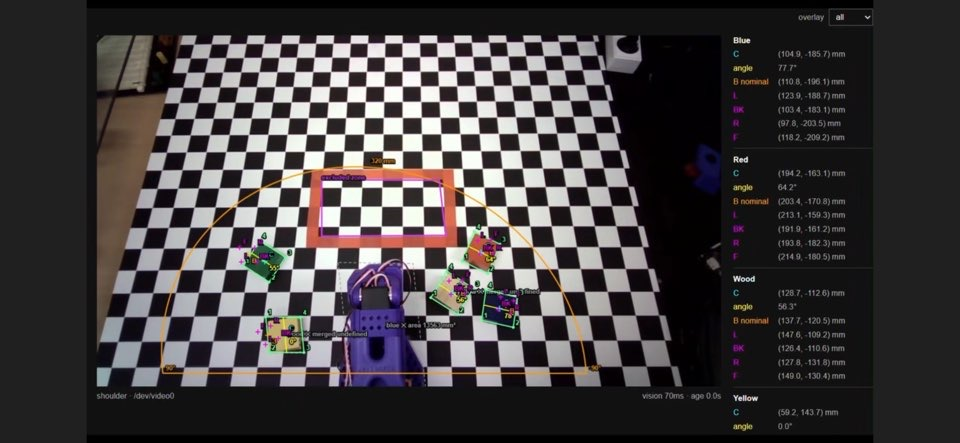
\includegraphics[width=0.7\linewidth]{camera_overlay}
\caption{관제 화면의 파지 방향 표시 예. 최종 방향 계산은 블록의 회전 사각형 방향과 베이스 중심 작업 영역의 접선을 이용하며, 화면의 선은 실제 턱 위치를 검출한 결과가 아니다.}
\label{fig:camera-overlay}
\end{figure}

관제 오버레이와 런타임 IK는 같은 정사각형 대칭 방향 선택 함수를 사용한다. 기본 파지 경로는 최초 관측으로 만든 후보를 실행하며, 파지 직전 실제 턱 위치를 재검출하여 XY를 보정하는 폐루프는 포함하지 않는다.

\subsection{도달성 검사와 접근 높이}
IK 결과는 모델 좌표에서의 위치 오차와 기울기 오차를 확인한 후 사용한다. 실행 전 계획의 허용 오차는 위치 15\,mm, 기울기 $6^\circ$로 설정하였다. 높은 접근점이 관절 한계에 걸릴 수 있으므로 최소 높이와 탐색 간격을 두고 가능한 접근 높이를 찾는다.

위치 15\,mm는 모델 안에서 계획 후보를 거르는 허용값이며, 실제 파지 여유를 측정한 값은 아니다. 그리퍼 개방 명령도 정규화 위치값이어서 실제 턱 간격으로 바로 환산할 수 없다. 따라서 IK 결과를 통과한 뒤에도 센서로 파지 상태를 확인한다.

인식 경로는 반경 320\,mm의 작업 영역 필터로 제어 대상을 제한한다. 이후 각 목표의 높이와 방향에 대해 IK를 풀어 실행 가능성을 판단한다. 관측 범위와 자세별 도달성을 두 단계로 검사하는 구조이다.

\subsection{측정 자세에서 시작하는 관절 보간}
웨이포인트 사이의 동작은 관절 공간에서 보간한다. 시작 자세 $\boldsymbol{q}_0$는 직전에 보낸 명령이 아니라 현재 측정값이며, 목표를 $\boldsymbol{q}_1$이라 하면 보간점은 다음과 같이 표현할 수 있다.
\begin{equation}
\boldsymbol{q}(\alpha)=(1-\alpha)\boldsymbol{q}_0+\alpha\boldsymbol{q}_1,
\qquad 0\leq\alpha\leq1.
\end{equation}
보간 과정에서 제어 주기(틱)당 관절 변화량을 제한하고, 로봇 입출력 단계의 상대 목표 클램프를 추가 적용한다. 측정 자세에서 시작하면 이전 동작이 목표에 충분히 도착하지 못한 경우에도 다음 궤적이 실제 자세와 다른 위치에서 시작해 급격한 명령 변화가 발생하는 것을 줄일 수 있다.

\begin{table}[htbp]
\centering
\caption{관절 제어와 파지 확인의 주요 설정값}
\begin{tabularx}{\linewidth}{@{}L{0.38\linewidth}L{0.19\linewidth}Y@{}}
\toprule
항목 & 설정값 & 의미 \\
\midrule
궤적 갱신 주파수 & 45\,Hz & 명령 생성의 목표 주파수 \\
틱당 일반 관절 변화 상한 & $2^\circ$ & 보간 단계의 제한 \\
하강 틱 변화 상한 & $0.6^\circ$ & 느린 접근을 위한 제한 \\
상대 목표 클램프 & 10.0 & 장비 입출력 계층의 추가 제한 \\
그리퍼 개방/닫힘 목표 & 95.0 / 2.0 & 정규화 위치 명령 \\
빈손 위치 경계 & 12.0 & 현재 파지 판정 설정 \\
파지 최소 부하 & 200.0 & 서보 부하값 기준 \\
파지 표본 수 / 간격 & 5회 / 0.05초 & 위치·부하 평균 계산 \\
\bottomrule
\end{tabularx}
\end{table}

명령 생성 목표 주파수는 30\,Hz에서 45\,Hz로 바꾸었다. 초기 180초 제한 시험에는 변경 전 설정을 사용하였다.

\section{상태 제어와 미션별 배치 전략}
\subsection{후보 실행과 파지 검증}
PICK에서는 기본 후보와 회전 재시도 후보의 IK 도달성을 검사한 뒤 실행 가능한 후보를 시도한다. 하강이 막히면 그리퍼를 열린 상태로 유지한 채 상공으로 후퇴하고, 정상 하강 후 빈손으로 닫히면 그리퍼를 다시 열고 후퇴하여 다음 후보를 시도한다. 후보를 소진하거나 개별 동작의 시간 제한에 걸리면 재선택 또는 순회 보류로 이어진다. PICK 내부의 후보 변경과 FSM의 대상 재선택은 서로 다른 복구 단계이다(그림~\ref{fig:pick-check}).

\begin{figure}[htbp]
\centering
\begin{tikzpicture}[
box/.style={draw,rounded corners,text width=3.7cm,minimum height=10mm,align=center,font=\small},
decision/.style={draw,diamond,aspect=2.6,text width=2.35cm,align=center,inner sep=1pt,font=\small},
arr/.style={-{Latex},thick}]
\node[box] (plan) at (0,0) {기본/회전 후보 계산};
\node[decision] (reach) at (0,-1.6) {도달 가능한\\후보 있음?};
\node[box] (attempt) at (0,-3.3) {정상 하강 후\\그리퍼 닫힘};
\node[decision] (held) at (0,-5.1) {$\bar p>12$ 그리고\\$\overline{|L|}\ge200$?};
\node[box] (success) at (0,-6.9) {PICK 통과\\필요시 후퇴 후 VERIFY 재확인};
\node[box,text width=2.8cm] (fail) at (5.1,-1.6) {PICK 실패\\재선택 / 순회 보류};
\node[decision] (more) at (5.1,-5.1) {남은 도달\\후보 있음?};
\draw[arr] (plan)--(reach);
\draw[arr] (reach)--node[right,font=\scriptsize]{예}(attempt);
\draw[arr] (reach)--node[above,font=\scriptsize]{아니오}(fail);
\draw[arr] (attempt)--(held);
\draw[arr] (held)--node[right,font=\scriptsize]{예}(success);
\draw[arr] (held)--node[above,font=\scriptsize]{아니오}(more);
\draw[arr] (more.north)--node[right,font=\scriptsize]{아니오}(fail.south);
\draw[arr] (more.north west)|-node[pos=0.75,above,font=\scriptsize]{예: 다음 후보}(attempt.east);
\end{tikzpicture}
\caption{PICK의 후보 선택과 정상 하강 후 센서 판정. 하강이 막힌 후보는 그리퍼를 닫지 않고 후퇴하여 다음 후보로 넘어간다. $\bar p$와 $\overline{|L|}$은 위치와 절대 부하의 표본 평균이며, 표시한 임계값은 평가에 사용한 설정이다. 개별 동작 시간 초과는 PICK 실패로 처리하며, 외부 180초 종료와 구분한다.}
\label{fig:pick-check}
\end{figure}

파지 판정에는 다섯 번 측정한 그리퍼 위치와 절대 부하의 평균을 사용하며 두 조건을 모두 만족해야 한다. VERIFY에서도 같은 조건을 검사하여 빈손 상태가 운반으로 이어지지 않게 한다. 실제 파지와 빈손 닫힘을 비교한 관찰은 절~\ref{sec:physical-grasp}에 제시한다.

\FloatBarrier
\subsection{추가 관측: 손목 영상과 마커 위치 추정}
\label{sec:additional-observation}
손목 카메라는 관제 영상과 데이터 수집에 활용하였다. 추가 관측 기능인 색상 게이트는 손목 영상에서 대상 색상이 검출되지 않으면 파지를 시작하지 않도록 하며, 미션 평가의 실제 제어에 적용하였다.

\begin{figure}[htbp]
\centering
\begin{subfigure}{0.48\linewidth}
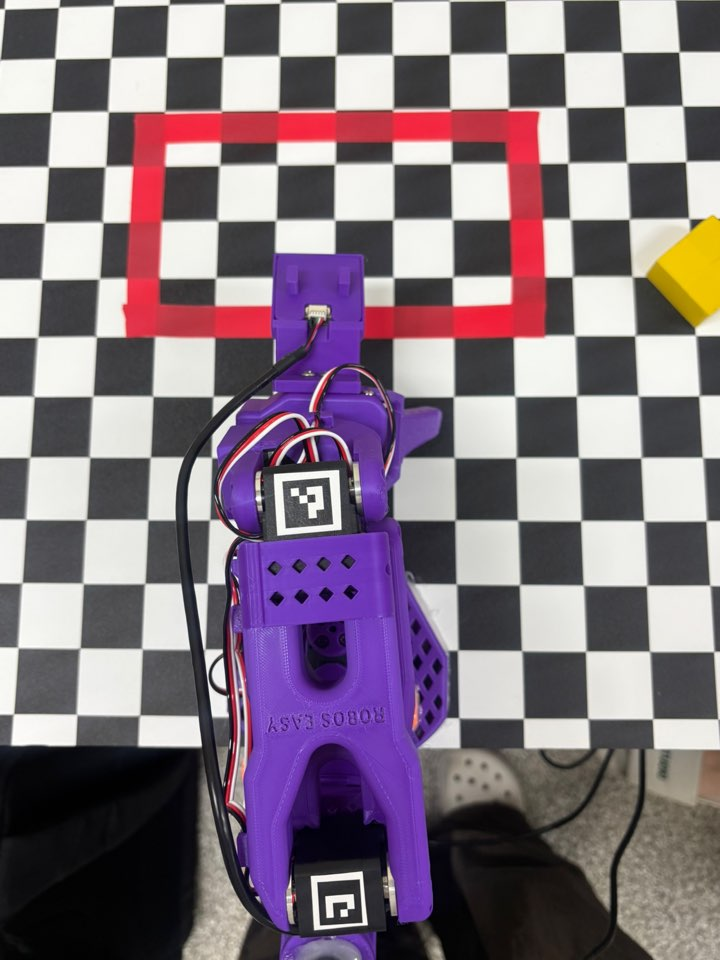
\includegraphics[width=\linewidth]{wrist_camera_mount}
\caption{그리퍼에 재장착한 손목 카메라}
\end{subfigure}\hfill
\begin{subfigure}{0.48\linewidth}
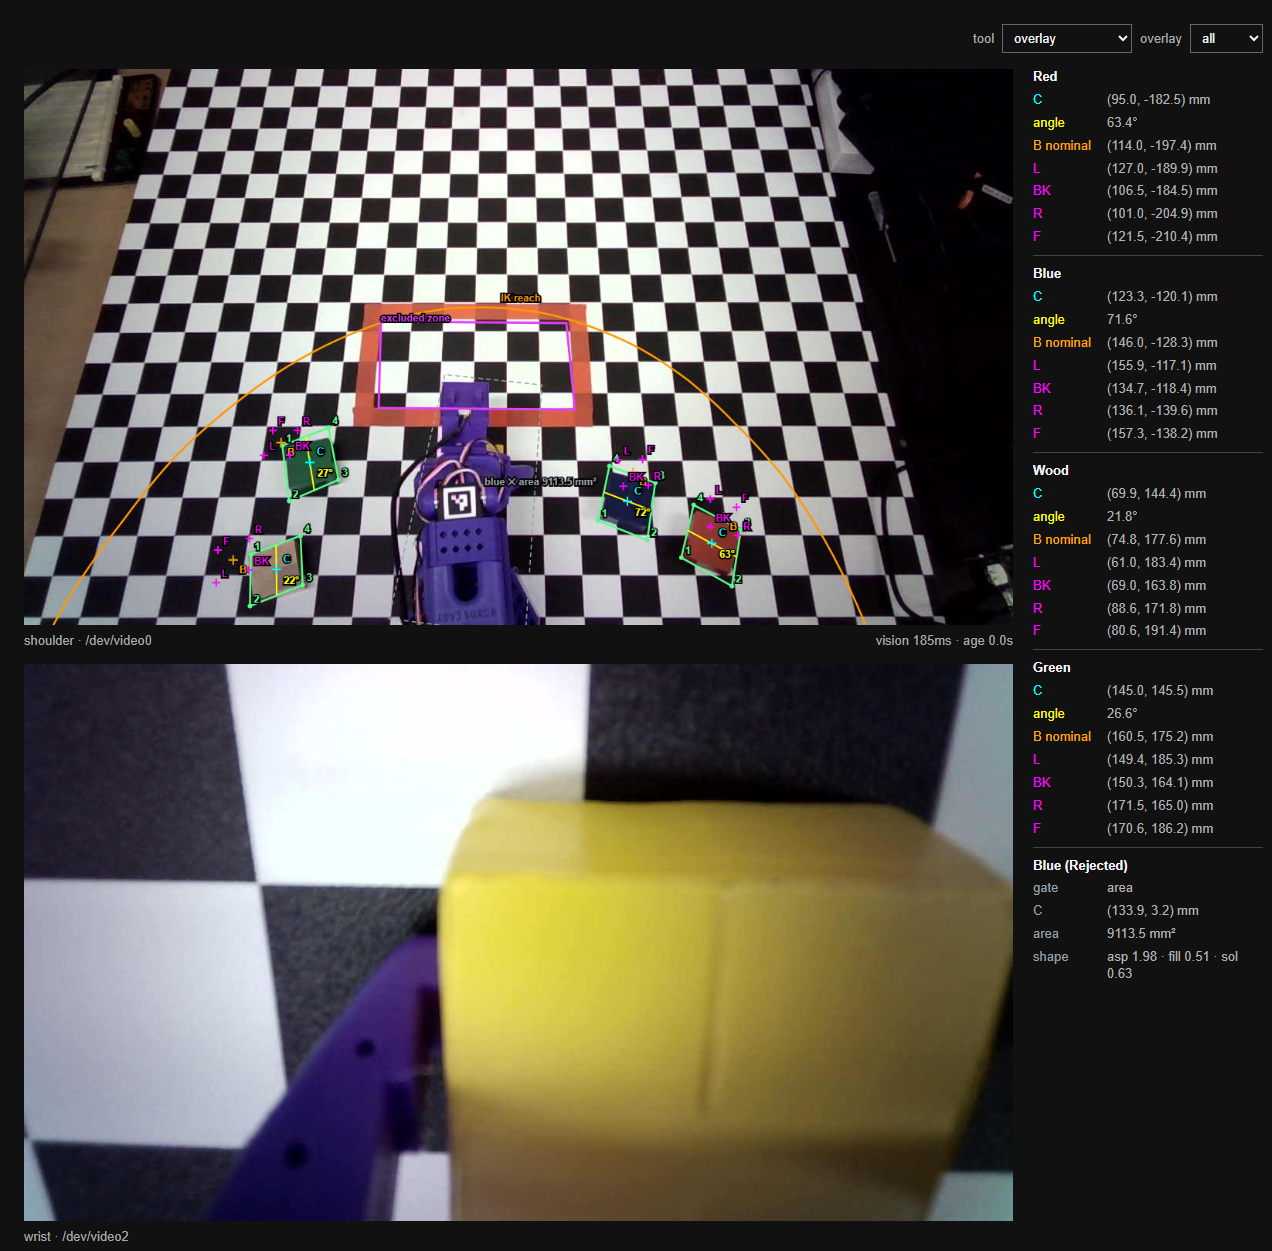
\includegraphics[width=\linewidth]{wrist_camera_view}
\caption{관제 화면의 어깨(위)·손목(아래) 카메라 동시 표시}
\end{subfigure}
\caption{손목 카메라 장착과 관제 화면. 손목 영상은 관제·데이터 수집에 사용하며, 추가 색상 게이트의 입력으로도 활용하였다.}
\label{fig:wrist-camera}
\end{figure}

그리퍼에는 ArUco 마커를 부착하여 위치 추정을 실제 제어 실험에 적용하였다. 마커 기반 위치 추정은 상단 영상의 블록 검출과 함께 사용하는 추가 관측 기능이다. 추정 좌표를 자동 수집 데이터의 필드로 저장하고 활용하는 작업은 후속 과제로 남았다.

\begin{figure}[htbp]
\centering
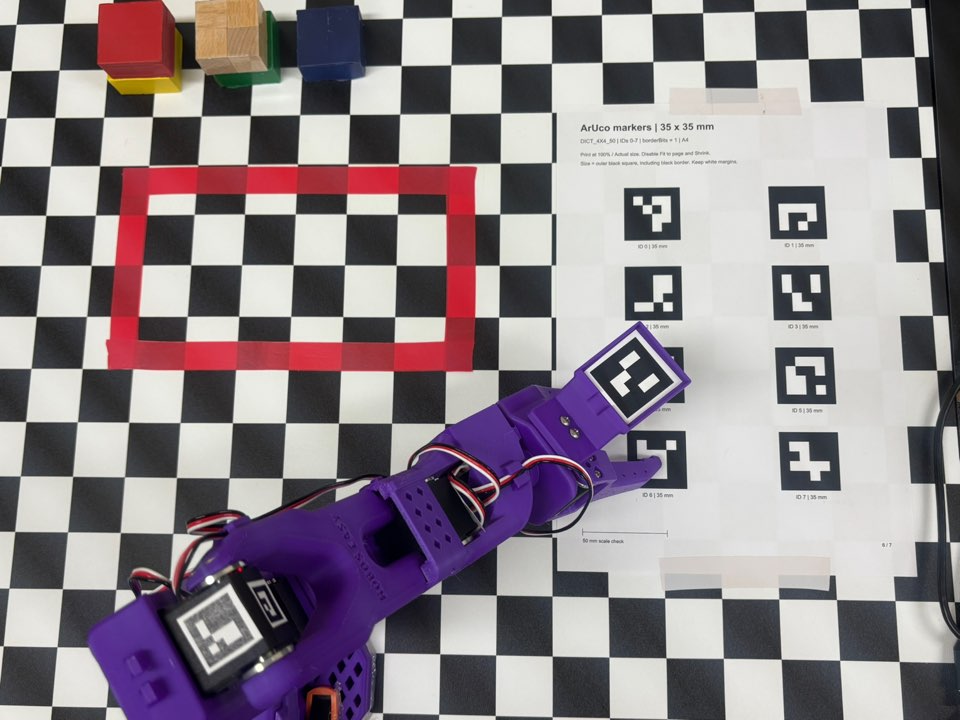
\includegraphics[width=0.62\linewidth]{aruco_markers}
\caption{그리퍼에 부착한 ArUco 마커(35$\times$35\,mm)와 마커 시트, 체커보드, 대상 블록. 상단·하단 두 지점에 마커를 부착하여 그리퍼 자세를 함께 추정할 수 있도록 하였다.}
\label{fig:aruco}
\end{figure}
\FloatBarrier

\subsection{1차 미션: 지정 영역의 동적 슬롯 배치}
1차 미션은 지정 영역 내부에 먼 행 세 개와 가까운 행 두 개의 슬롯을 구성한다. 영역 네 꼭짓점과 정규화 좌표를 이용하여 슬롯 중심을 계산하고, 각 슬롯의 해제점과 상공 자세를 IK로 구한다. 기본 정규화 좌표는 $(0.14,0.20)$, $(0.50,0.20)$, $(0.80,0.20)$, $(0.32,0.76)$, $(0.68,0.76)$이다. 선택한 색은 예약한 슬롯을 유지하여 재시도 때 배치 위치가 불필요하게 바뀌는 것을 줄인다.

\begin{figure}[htbp]
\centering
\begin{tikzpicture}[x=0.055cm,y=0.055cm]
\draw[thick] (0,0) rectangle (200,100);
\draw[<->] (0,-12)--node[below]{200\,mm}(200,-12);
\draw[<->] (-12,0)--node[left,rotate=90,anchor=south]{100\,mm}(-12,100);
\foreach \x/\y/\name in {28/80/0,100/80/1,160/80/2,64/24/3,136/24/4}{
\draw[fill=black!6] (\x-20,\y-20) rectangle (\x+20,\y+20);
\fill (\x,\y) circle (1.5);
\node[above,font=\small] at (\x,\y+3) {\name};}
\node at (100,115) {먼 행};
\node at (100,-30) {로봇 쪽 / 가까운 행};
\end{tikzpicture}
\caption{200\,$\times$\,100\,mm 지정 영역의 3+2 슬롯 설계. 사각형은 40\,mm 블록의 명목 크기, 숫자는 슬롯 번호이다.}
\label{fig:slots}
\end{figure}

운반 경로는 파지 위치와 배치 위치의 높이·도달성을 고려하여 계산한다. 필요하면 베이스 쪽으로 당긴 경유점에서 더 높은 통과 자세를 만든 후 목표 슬롯 상공으로 이동한다. 해제 높이는 캘리브레이션의 평균 파지 높이에 가정한 여유 5\,mm를 더해 계산한다.

1차 미션은 HOME에서 새 프레임을 받아 지정 영역 밖의 검출이 연속 5초 동안 없으면 완료 상태로 전이한다. 중복되거나 오래된 프레임은 완료 시간에 누적하지 않는다. 이 판정은 관측된 블록 중심에 의존하므로, 검출 누락과 실제 경계 걸침을 포함한 물리적 완료 판정에는 한계가 있다.

\subsection{재시도와 실행 종료}
대상별 재시도 횟수는 한 순회 안에서만 제한한다. 남은 색이 모두 보류되면 시도 기록을 유지한 채 새 순회를 시작한다. 1차 미션 실행기는 내부 FSM 시간 제한을 비활성화한 상태로 외부 타이머를 사용하였다. 따라서 순회가 반복될 때 늘어나는 누적 재시도 시간은 외부 제한으로 관리한다.

제한시간 시험에서는 외부 타이머가 180초에 종료 신호를 보낸다. 종료 신호를 받은 뒤 그리퍼 개방과 홈 복귀를 시도하므로 전체 모터 동작이 180초 안에 끝나는지는 별도로 판정해야 한다.

\subsection{2차 미션: 적재 계획과 해제 전략}
2차 미션은 1차 미션의 대상 선택·파지·확인 흐름을 공유하고 목적지를 한 적재 좌표로 바꾼다. 계획기는 등록 영역 안의 좌표와 캘리브레이션의 파지 높이, 명목 블록 높이로 층별 접근·해제 자세를 IK로 계산한다. 평가에서는 접촉 하강을 비활성화하고, 계획한 해제 자세에 도달하면 그리퍼를 열어 다음 순회로 넘어갔다.

초기에는 관절 키프레임과 부하 변화로 접촉을 감지하는 하강 전략을 구성했으나, 최종 적재 시험에는 계산한 자세에서 직접 해제하는 방식을 사용하였다. 명목 높이와 배치 횟수로 만든 계획은 실제 타워 높이의 측정값이 아니므로, 해제 후 블록의 안착과 유지 상태를 별도로 관찰해야 한다.

적재 평가는 5단을 목표로 한 20회의 시험에서 수행 중 도달한 최대 높이를 집계하였다. 결과는 절~\ref{sec:stack-results}에 제시한다.

\subsection{Task3: 데이터셋 자동 수집 구조}
Task3은 CV+IK의 실행 중 관측과 동작을 기록하여 리더암 조작 없이 학습용 에피소드를 수집한다. 센서값과 검출 결과로 대상 선택·파지·배치를 판정하는 기존 실행 루프에 기록 기능을 연결하였다.

로봇 I/O 경계에 \texttt{RecordingRobotIO} 데코레이터를 두었다. 명령 직전의 관측과 안전 제한을 거쳐 실제 전송된 액션을 한 프레임으로 묶어 LeRobotDataset의 관절 상태, 설정한 카메라 영상, 액션과 작업 지시 형식으로 저장한다. PICK/VERIFY/TRANSPORT 코드는 1차 미션과 같다. 학습 자료의 행동값이 로봇 명령과 일치하도록 안전 제한 전의 요청값 대신 실제 전송값을 기록한다.

Task3의 에피소드는 대상 선택을 마친 HOME 자세에서 시작하여 파지$\to$운반$\to$배치$\to$HOME 복귀로 끝난다. 대상 선택을 위한 카메라 대기는 기록 구간에서 제외하며, 센서 파지 확인을 통과하고 배치와 복귀까지 끝난 사이클을 저장한다. 개별 에피소드의 실제 안착 여부를 독립 영상 판정한 라벨과는 구분한다. 1차/2차 미션과 달리 회전·위치 후보로 재시도하지 않고 최초 파지 1회만 시도하여, 복구 동작을 제외한 실행을 수집하도록 설계하였다. 지정 영역 밖의 블록이 5초간 탐지되지 않으면 한 라운드가 끝난 것으로 보고 작업자에게 블록 재배치를 요청한다.

저장 자료는 관절·행동 데이터, 카메라 영상과 에피소드 메타데이터로 구성된다(표~\ref{tab:task3-structure}).

\begin{table}[htbp]
\centering
\caption{자동 수집 데이터의 구성}\label{tab:task3-structure}
\begin{tabularx}{\linewidth}{@{}L{0.22\linewidth}L{0.20\linewidth}Y@{}}
\toprule 자료 & 형식 & 저장 내용 \\
\midrule
관절·행동 & parquet & 관측한 관절 상태와 실제 전송한 액션 \\
카메라 영상 & MP4 & 설정한 카메라의 관측 영상 \\
메타데이터 & JSON, parquet & 에피소드 구분, 작업 지시와 통계 \\
\bottomrule
\end{tabularx}
\end{table}

\subsection{안전 처리와 실행 기록}
안전장치는 관절 보간의 변화량 제한, 상대 목표 클램프, IK 게이트와 파지 확인에 나누어 적용하였다. 하강 중 턱이 물체에 걸렸는데도 명령을 계속 보내면 블록을 밀거나 팔이 구속될 수 있다. 측정 관절과 명령의 차이를 검사해 하강을 중단하며, PICK에서는 그리퍼를 닫지 않고 상공으로 후퇴한 뒤 다음 후보를 시도한다. 하강 중 명령 추종 오차의 상한은 8.0, 하강 종료 시 목표 미도달 판정 경계는 4.0으로 조정하였다. 두 값은 로봇 입출력의 관절 명령 단위를 따르는 설정값이다.

정상 종료와 예외 발생 시 모두 그리퍼 개방, 홈 복귀와 연결 해제를 시도하도록 종료 절차를 구성하였다. 통신이나 장비 오류가 지속되면 정리 동작이 실패할 수 있으므로 오류와 최종 상태를 함께 기록한다. 연결 해제 후에는 팔의 자세 유지를 위해 토크를 유지한다. 모터를 구동하지 않는 사전 경로 검사와 실제 장비 시험은 별도로 수행하였다.

실험마다 적용 설정, 대응점·관절값, 상태 전이와 단계별 사진을 저장하여 실패 단계와 실행 조건을 추적하였다.

\Needspace{27\baselineskip}
\section{개발 일정과 구성원별 수행 내용}
\subsection{개발 경과}
개발 경과와 산출물은 표~\ref{tab:timeline}과 같다.
\begin{longtable}{@{}L{0.20\linewidth}L{0.70\linewidth}@{}}
\caption{주요 개발 경과와 산출물}\label{tab:timeline}\\
\toprule 시기 & 수행 내용 및 산출물 \\\midrule
\endfirsthead
\toprule 시기 & 수행 내용 및 산출물 \\\midrule
\endhead
3--5월 & 초기 물체 수집 주제 검토, 시스템 구상과 착수보고서 작성 \\
6월 & SO-101 과제로 변경, 장비 수령, 리더·팔로워 환경과 데이터 수집 기반 구성 \\
7월 & SmolVLA·ACT 학습·실행, 원격 추론과 카메라 도구 개발, 중간보고서 작성 \\
8월 초 & 산업체 서면 자문, 구현·검증 구분과 접근법 선정·비용 비교 의견 수렴 \\
8월 말 & CV+IK 파지 경로, 캘리브레이션·기구학 도구 개발, 손목 방향과 위치 오차 분석 \\
9월 / 통합 시연 & 검출과 3+2 슬롯 배치 기능 통합, 1차 미션 시연 \\
9월 / 실기 평가 & 카메라 재고정, 9점 캘리브레이션, 제한시간·단일 블록 시험, 실험 기록 정리 \\
9월 / 결과 정리 & 최종 시스템 결과 분석, 최종보고서 작성과 자문의견 반영 \\
\bottomrule
\end{longtable}

\Needspace{31\baselineskip}
\subsection{역할 분담과 공동 작업}
비전과 미션 제어, 관제·캘리브레이션 도구, 평가와 기술 문서를 나누어 담당했으며 장비 통합과 결과 검토는 공동으로 진행하였다(표~\ref{tab:roles}).

\begin{longtable}{@{}L{0.14\linewidth}L{0.82\linewidth}@{}}
\caption{구성원별 수행 내용}\label{tab:roles}\\
\toprule 구성원 & 수행 내용 \\\midrule
\endfirsthead
\toprule 구성원 & 수행 내용 \\\midrule
\endhead
윤민석 & 블록별 채도·밝기와 영역 필터 조정(도달 범위 밖·지정 영역 내 블록 제외). 파지·적재 위치의 mm 단위 보정과 블록 각도 기반 그리퍼 회전 정렬.\newline
손목 서보 과열 분석과 제어 개선. 파지 실패 재시도, 성공 후 운반과 미션 종료 조건 구현.\newline
1차 미션 제어 경로 통합 및 졸업과제 포스터 제작. \\
이동근 & FSM 파지 조건과 도달 실패 시 대체 후보 처리 보완. 카메라 웹 뷰어 및 검출·파지 후보·FK 위치의 실시간 시각화.\newline
대응점·관절값 기록과 수집 재개를 지원하는 캘리브레이션 도구 개발. 영상 변화 감지에 따른 실험 이미지 자동 저장 구현.\newline
LeRobot 의존성과 uv 환경 통합, Python CLI 실행 도구 정리. 설정·로그·캘리브레이션 자료 관리 및 중간·최종보고서 작성. \\
김주환 & SmolVLA·ACT의 한계 분석과 규칙 기반 FSM 전환 근거 정리. 정량 평가 체계 및 실행 기록 양식 작성·배포.\newline
캘리브레이션 시행착오 문서화·공유. 실행 환경 통합 시험과 미션 실행 검증.\newline
코드 검토, 개발 규칙·변경 이력 관리 및 최종보고서·최종 시연 PPT 작성. \\
공동 수행 & 실제 장비 통합, 데이터 수집과 실패 관찰. 접근법 논의, 결과 검토와 보고 자료 정리. \\
\bottomrule
\end{longtable}
\FloatBarrier

\chapter{연구 결과 분석 및 평가}
\section{실험 환경과 평가 방법}
평가는 소프트웨어 구성, 좌표·센서 측정, 단일 블록 실기 동작, 전체 미션의 관찰을 구분하여 수행하였다. 본 장은 최종 CV+IK 경로의 자료를 중심으로 하며, 3장에 제시한 ACT의 58\%를 최종 시스템의 평가값으로 사용하지 않는다. 각 실험에서 확인한 범위와 남은 조건을 결과와 함께 제시한다.

9월 8일 기록에는 카메라 재고정과 단축 드리프트 검사, 아홉 점 캘리브레이션, 1차 미션의 외부 시간 제한 시험, 노란 블록의 위치 변경 후 파지·운반 관찰이 포함되어 있다. 시험 중 기본 설정을 변경하거나 실행 인자로 덮어쓴 항목이 있으므로, 저장소의 최신 YAML만으로 당시 실행을 재구성하지 않는다. 특히 배치 슬롯 보정과 모션 주파수를 구분하였다.

\begin{longtable}{@{}L{0.18\linewidth}L{0.32\linewidth}L{0.40\linewidth}@{}}
\caption{평가 단위와 성공 판단의 구분}\label{tab:eval-definitions}\\
\toprule 평가 단위 & 판단 대상 & 필요한 근거 \\\midrule
\endfirsthead
\toprule 평가 단위 & 판단 대상 & 필요한 근거 \\\midrule
\endhead
블록 검출 & 실제 블록의 검출·누락·오검출 & 정답이 표시된 프레임과 검출 결과. 현재 집계 추가 필요 \\
좌표 변환 & 대응점과 예측 위치의 차이 & 적합 잔차, LOO, 대응점 및 캘리브레이션 조건 \\
단일 파지 & 물체를 물고 들어 올렸는가 & 그리퍼 위치·부하, 단계 사진과 관찰 \\
단일 배치 & 목표 영역에 내려놓았는가 & 해제 전후 영상, 실제 경계와 블록 상태 \\
1차 전체 & 180초 내 다섯 블록 배치 & 시작 배치, 종료 시각과 다섯 블록의 실제 위치 \\
2차 전체 & 300초 내 적재와 5초 유지 & 적재 블록 수, 해제 이후 연속 영상과 유지시간 \\
소프트웨어 & 계약·상태 흐름·계산의 동작 & 단위·통합 테스트 기록. 실기 성능과 별도 평가 \\
\bottomrule
\end{longtable}

파지 부하값은 힘 단위로 교정되지 않았고, FK 좌표는 측정 관절값을 URDF로 변환한 값이다. 따라서 부하 500을 특정 파지력으로 환산하거나, FK 목표 오차를 물체와 턱의 실제 거리 오차로 표현하지 않는다. 다음 절의 수치는 이 정의에 따라 해석한다.

\section{캘리브레이션과 위치 오차 분석}
\subsection{아홉 점 적합 결과}
9월 8일 채택된 캘리브레이션의 대응점은 아홉 개이다. 첫 번째 점은 재시도한 \texttt{P1\_retry2}를 사용하였고 나머지는 P2--P9이다. 적합 보고서의 RMS는 8.18\,mm, 최대 잔차는 14.51\,mm, 최대 LOO 오차는 26.64\,mm이다. 적합기의 기준인 RMS 5\,mm 미만과 최대 LOO 8\,mm 미만을 모두 만족하지 못하였다.

\begin{table}[htbp]
\centering
\caption{9월 8일 채택한 아홉 점의 적합 잔차와 LOO 오차}\label{tab:calibration}
\begin{tabular}{@{}lrr@{}}
\toprule 대응점 & 적합 잔차 (mm) & LOO 오차 (mm) \\
\midrule
P1 (retry2) & 6.05 & 26.64 \\
P2 & 6.05 & 17.54 \\
P3 & 4.66 & 7.64 \\
P4 & 14.51 & 21.04 \\
P5 & 4.83 & 7.17 \\
P6 & 8.44 & 20.13 \\
P7 & 5.12 & 7.58 \\
P8 & 12.34 & 16.44 \\
P9 & 4.82 & 17.08 \\
\midrule
최대 & 14.51 & 26.64 \\
\bottomrule
\end{tabular}
\end{table}

\begin{figure}[htbp]
\centering
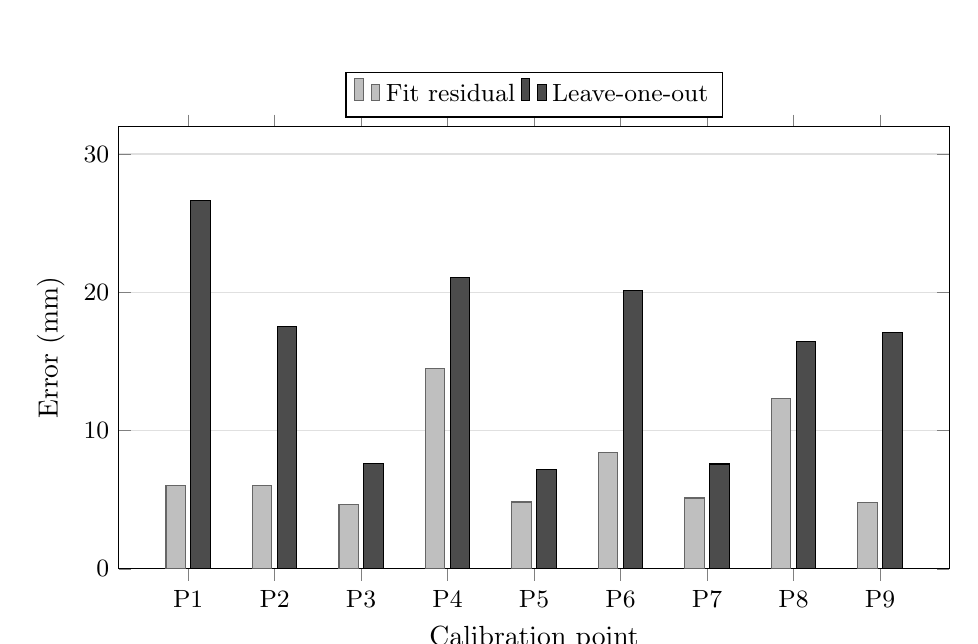
\begin{tikzpicture}
\begin{axis}[width=\linewidth,height=7.2cm,ybar,bar width=7pt,
symbolic x coords={P1,P2,P3,P4,P5,P6,P7,P8,P9},xtick=data,
ymin=0,ymax=32,ylabel={Error (mm)},xlabel={Calibration point},
legend style={at={(0.5,1.02)},anchor=south,legend columns=2,font=\small},
ymajorgrids=true,grid style={black!12},tick label style={font=\small}]
\addplot[fill=black!25,draw=black!60] coordinates {(P1,6.05)(P2,6.05)(P3,4.66)(P4,14.51)(P5,4.83)(P6,8.44)(P7,5.12)(P8,12.34)(P9,4.82)};
\addplot[fill=black!70,draw=black] coordinates {(P1,26.64)(P2,17.54)(P3,7.64)(P4,21.04)(P5,7.17)(P6,20.13)(P7,7.58)(P8,16.44)(P9,17.08)};
\legend{Fit residual,Leave-one-out}
\end{axis}
\end{tikzpicture}
\caption{표~\ref{tab:calibration}의 오차 비교. P1은 재시도 점이다. 적합에 사용한 점의 잔차보다 LOO 오차가 크게 나타나는 점이 있어 새 위치에 대한 정확도를 별도로 확인해야 한다.}
\label{fig:fit}
\end{figure}

이 결과는 사용한 변환이 시험에 투입되었다는 사실을 보여주지만 품질 기준 통과를 뜻하지 않는다. 일부 점의 잔차가 작더라도 모든 위치에서 그 정도의 정확도를 기대할 수 없으며, 최대 LOO 오차는 블록 폭 40\,mm에 비해 작은 값이라고 보기 어렵다. 대응점을 추가하거나 제외할 때에는 적합 RMS 감소만으로 변경을 채택하지 않고, 별도 위치에서의 물리적 파지 결과와 함께 확인해야 한다.

같은 적합 보고서에 기록된 파지 높이는 평균 16.2\,mm, 표준편차 6.8\,mm, 범위 1.2--26.3\,mm이다. 이는 로봇 베이스 프레임에서 기록한 높이이며 테이블로부터 블록 높이 20\,mm와 동일한 값이 아니다. 높이와 자세의 일관성이 충분히 확보되었는지, FK 기준점이 실제 턱의 어느 지점에 대응하는지 추가 검토할 필요가 있다.

\subsection{카메라 드리프트의 단축 검사}
보관된 두 드리프트 CSV는 각각 약 60.5초 동안 12개 표본을 기록하였다. 각 표본의 p95는 그 시점에서 대응된 코너 변위의 95백분위값이다. 첫 기록에서 표본별 p95의 최댓값은 2.775\,pixel이었고, 재검사 기록에서는 0.514\,pixel이었다. 재검사 값은 세션 요약의 약 0.51\,pixel과 대응한다.

\begin{figure}[htbp]
\centering
\begin{tikzpicture}
\begin{axis}[width=\linewidth,height=6.8cm,xlabel={Elapsed time (s)},ylabel={Frame-wise p95 drift (px)},
xmin=0,xmax=65,ymin=0,ymax=3.2,grid=major,grid style={black!12},
legend style={font=\small,at={(0.5,1.02)},anchor=south,legend columns=3},
tick label style={font=\small}]
\addplot[black!70,mark=square*,thick] table[x=elapsed_s,y=p95_px,col sep=comma]{figures/drift_initial.csv};
\addplot[black,mark=*,thick] table[x=elapsed_s,y=p95_px,col sep=comma]{figures/drift_retry.csv};
\addplot[dashed,black,domain=0:65,samples=2] {2};
\legend{Initial,Retry,2 px reference}
\end{axis}
\end{tikzpicture}
\caption{보관된 단축 드리프트 검사의 표본별 p95. 두 기록은 각각 별도 검사의 경과시간을 나타내며 10분 검사를 수행한 결과가 아니다.}
\label{fig:drift}
\end{figure}

재검사에서 개별 코너의 최대 변위는 12.354\,pixel까지 기록되어 p95보다 훨씬 컸다. 이는 일부 대응 코너의 변동이 전체적인 변위와 다를 수 있음을 보여주므로, 최대값만으로 카메라 전체가 그만큼 이동했다고 판단하지 않는다. 반대로 낮은 p95만으로 장시간 강체 고정을 입증하지도 않는다. 검사 시간이 약 1분이기 때문에 설계상 요구한 10분 게이트는 미검증으로 남는다.

\subsection{서로 다른 위치 비교의 해석}
세션 요약에는 V1과 V2의 블록·FK 비교값 19.94\,mm와 7.11\,mm가 기록되어 있다. 두 값은 서로 다른 자세에서 얻은 관찰이므로 같은 조건의 보정 전후 비교가 아니다. 따라서 이를 보정으로 오차가 12.83\,mm 감소했다는 결과로 사용하지 않는다. 새로운 보정의 효과를 평가하려면 같은 물체 위치·방향과 카메라 조건에서 적용 여부만 바꾸어 반복해야 한다.

과거 설계 규칙은 주된 오차를 실제 기구와 URDF의 차이로 설명하고, 전환 정리 문서는 데이터 수집 과정의 측정 편차를 유력한 원인으로 설명하였다. 현재 자료만으로 어느 한 요인을 분리하여 확정하기 어렵다. 본 보고서는 위치별 오차와 실패를 관찰 결과로 제시하고, 기구학 모델, 물리적 턱 기준점, 수집 자세·높이 및 접촉 위치의 영향을 후속 분리 실험 대상으로 둔다.
\FloatBarrier

\section{CV+IK 실기 수행 결과}
\subsection{9월 2일 1차 미션 시연 영상}
팀 대화에는 9월 2일 1차 미션 성공 보고와 함께 실제 로봇 동작 영상이 공유되어 있다. 확보된 해당 파일의 재생시간은 약 105.59초이다. 초안 작성에서는 원본의 0, 15, 30, 45, 60, 75, 90, 104초 프레임을 추출하여 대표 진행 장면을 확인하였다. 블록을 순차적으로 집어 지정 영역 쪽으로 운반하고, 영상 후반에 여러 색의 블록이 영역 부근에 모이는 모습을 관찰할 수 있다.

\begin{figure}[htbp]
\centering
\begin{subfigure}{0.48\linewidth}
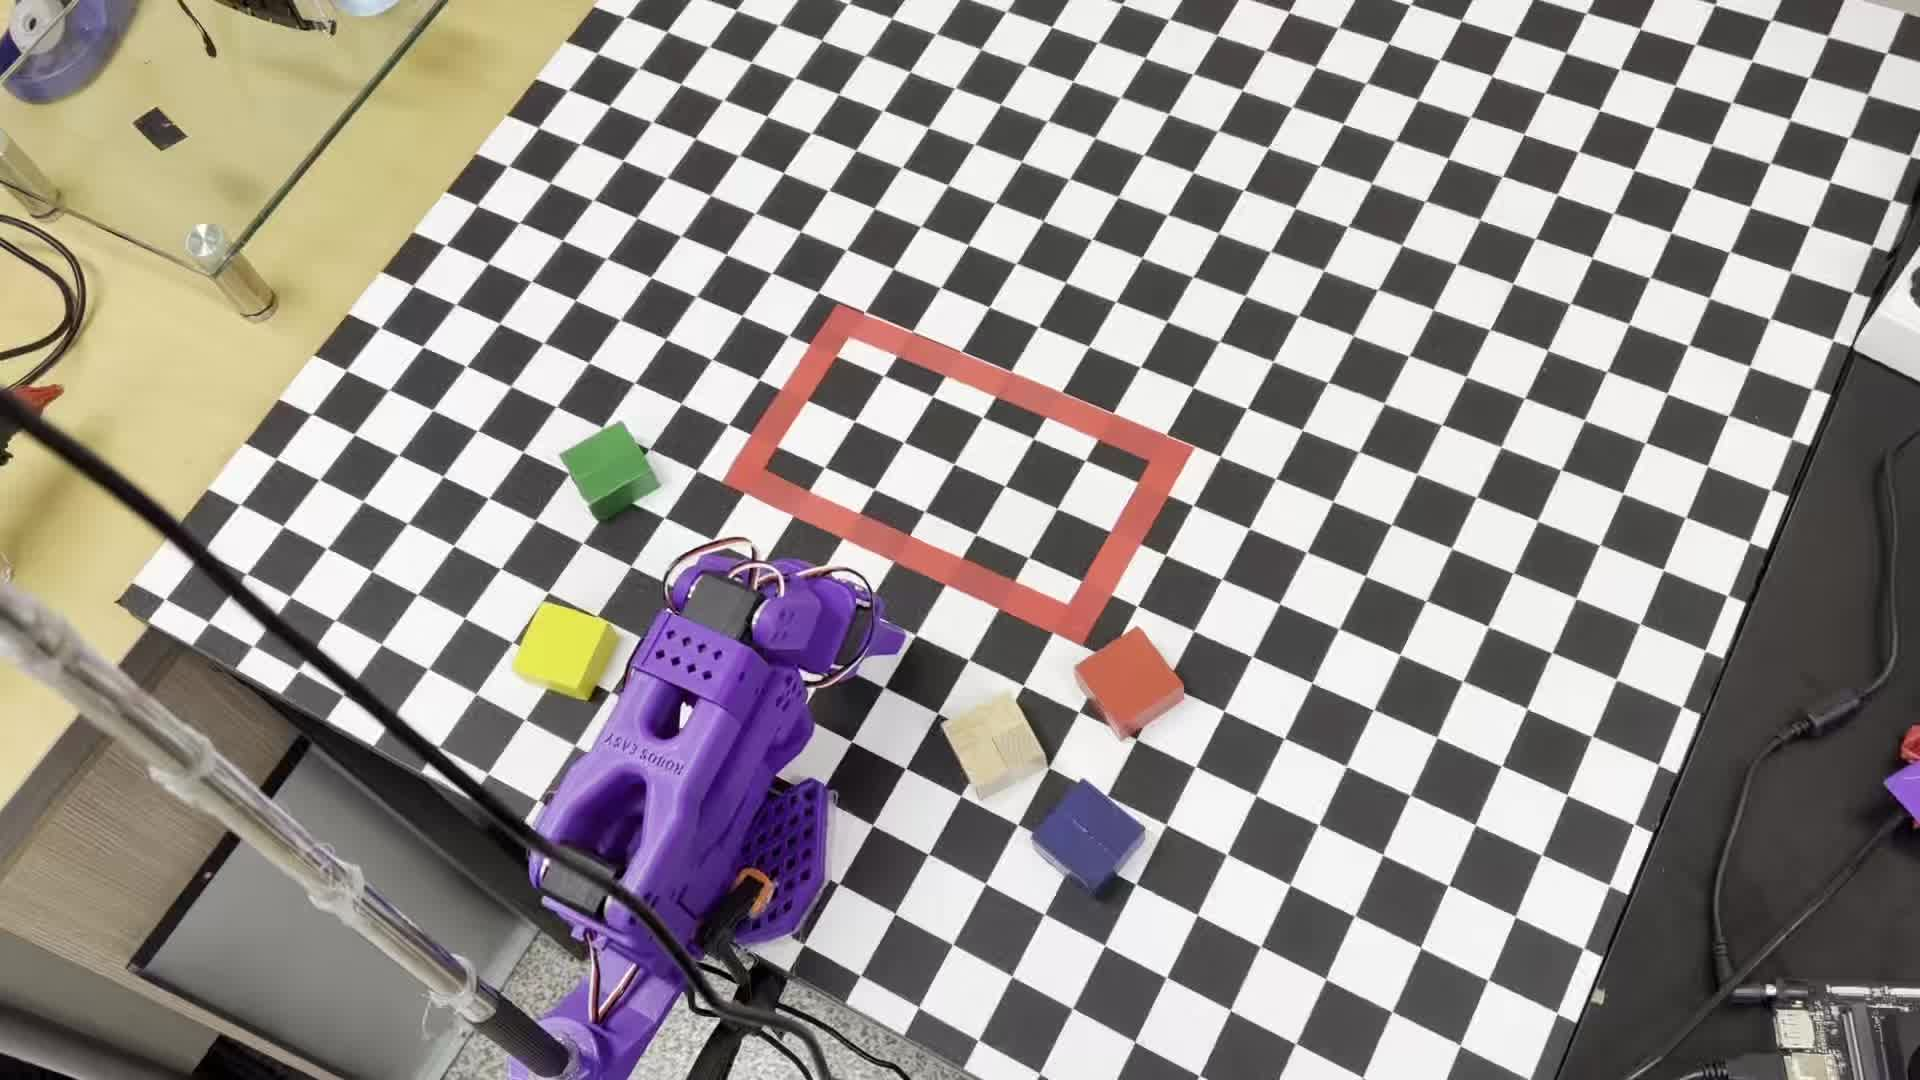
\includegraphics[width=\linewidth]{demo_000.jpg}
\caption{재생 위치 0초}
\end{subfigure}\hfill
\begin{subfigure}{0.48\linewidth}
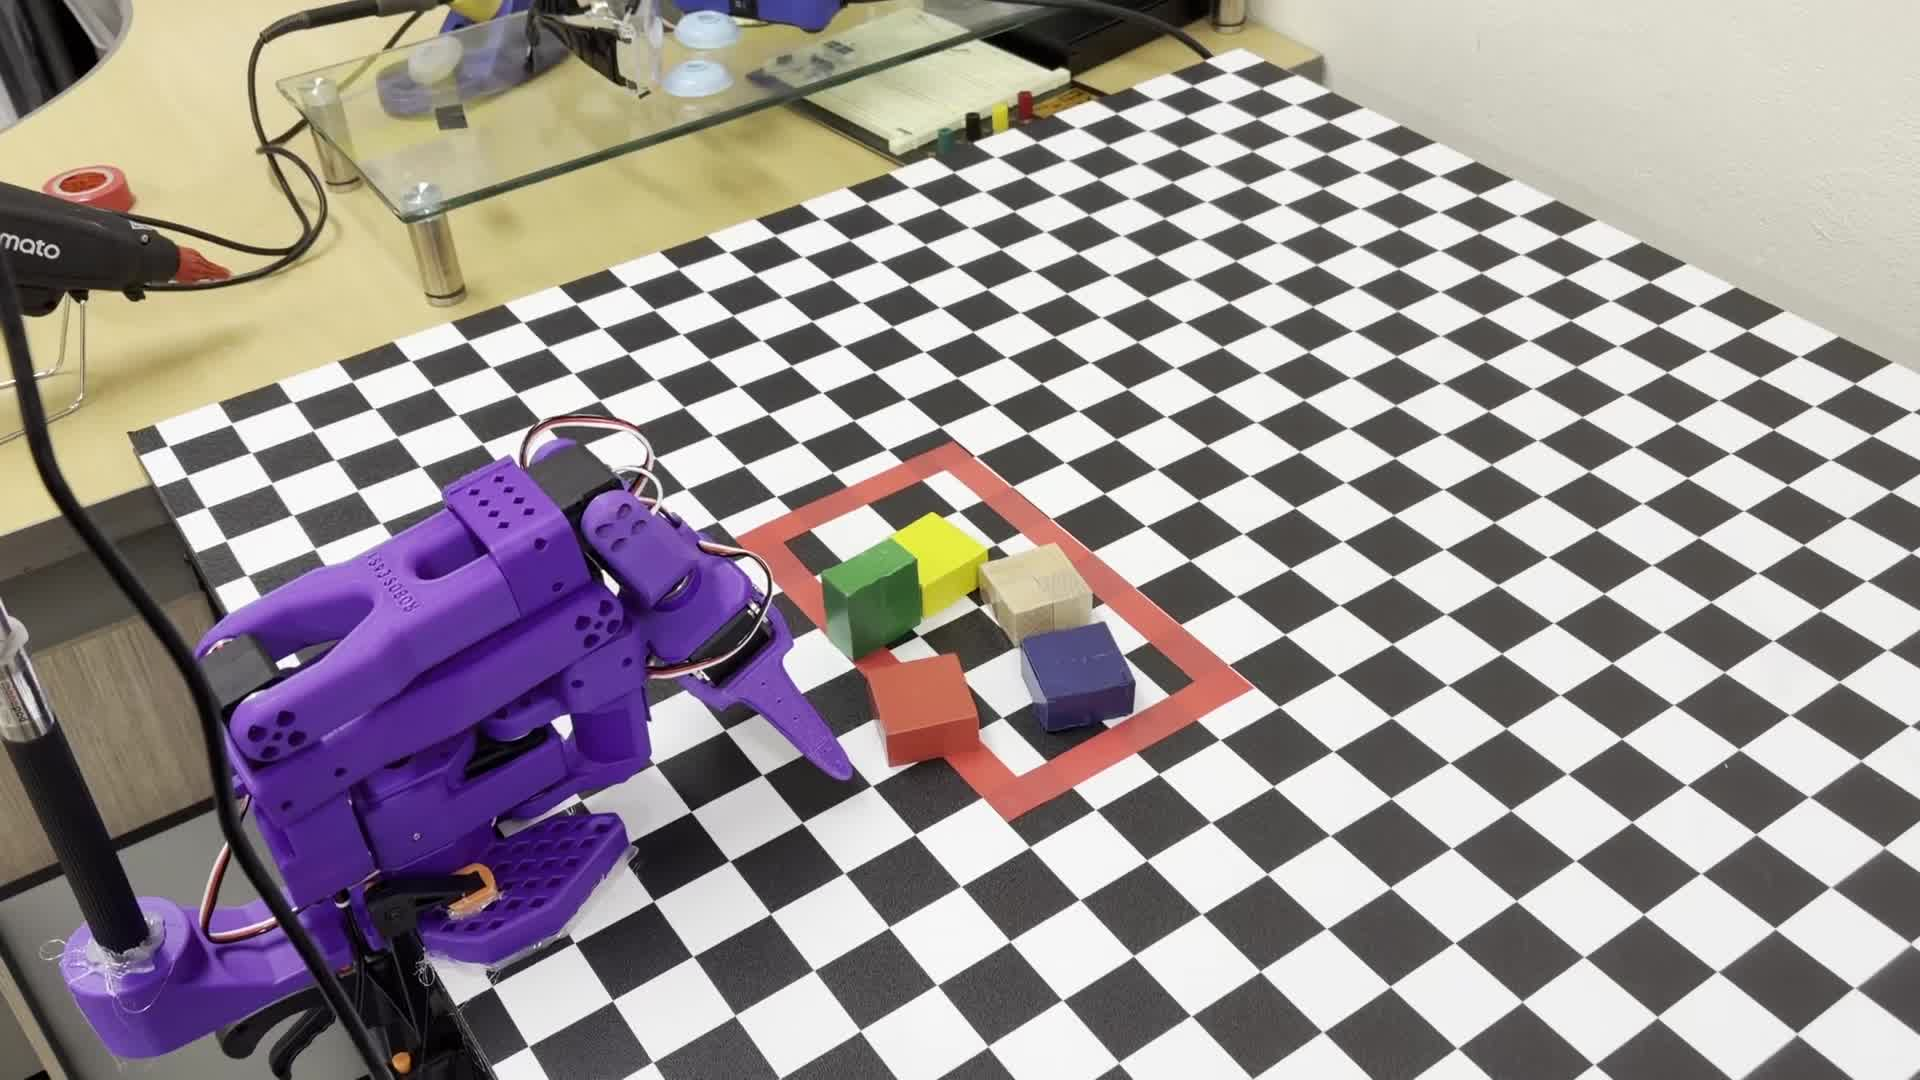
\includegraphics[width=\linewidth]{demo_104.jpg}
\caption{재생 위치 104초}
\end{subfigure}
\caption{9월 2일 공유 영상의 발췌 프레임. 표기한 시간은 파일 내 재생 위치이며 공식 미션 소요시간이 아니다.}
\label{fig:demo}
\end{figure}

이 자료는 실제 장비에서 CV+IK 기반 순차 조작을 수행한 시연 사례로 사용한다. 촬영 시작과 미션 시작의 일치 여부, 재생 속도·편집 여부, 경계 허용치의 실측 및 반복 횟수는 추가 확인이 필요하다. 일부 장면은 팔과 촬영 각도에 의해 블록이 가려져 있으므로, 발췌 프레임만으로 모든 블록의 경계 조건을 독립 판정하지 않는다. 파일 길이를 그대로 미션 완료시간으로 사용하거나 한 시연으로 전체 성공률을 산출하지 않는다.

\subsection{9월 8일 외부 시간 제한 시험}
별도의 1차 미션 시험은 180초 외부 제한을 사용하였다. 세션 기록에 따르면 네 번의 배치 동작을 수행했으나 파란 블록이 지정 영역 밖에 남았다. 따라서 해당 시험은 다섯 블록 전체 미션 성공으로 처리하지 않는다. 로그 마지막에는 실행 중 종료 신호에 따른 \texttt{KeyboardInterrupt}가 남아 있어, 정상 DONE 전이로 전체 목표를 달성한 로그와 구분된다.

이 시험에서는 슬롯의 기본 반경 보정 20\,mm가 dry-run에서 문제를 보여 다섯 슬롯 모두 0\,mm로 실행 인자를 덮어썼다. 저장된 YAML의 기본값은 그대로 유지되었다. 또한 시험 이후 모션 주파수를 45\,Hz로 변경하였으나 동일한 전체 미션을 변경된 주파수로 다시 시험한 기록은 이 세션에 없다. 그러므로 시연 영상과 제한시간 시험을 비교하여 주파수 변경이나 특정 보정의 효과를 계산할 수 없다.

\subsection{단일 노란 블록 파지와 위치 변경}
단일 블록 시험은 파지 센서, 계획 좌표와 단계 사진을 함께 제공한다. 첫 위치에서 노란 블록을 파지하고 들어 올리는 데 성공하였고, 이후 블록을 안쪽 위치로 운반하여 내려놓았다. 안쪽 위치의 기본 파지와 왼쪽 보정 재시도에서는 빈손으로 닫히는 결과가 관찰되었다. 표~\ref{tab:pick-results}는 원본 요약 JSON의 값을 반올림하여 나타낸 것이다.

\begin{table}[htbp]
\centering
\caption{9월 8일 노란 블록의 위치별 관찰}\label{tab:pick-results}
\begin{tabularx}{\linewidth}{@{}L{0.24\linewidth}YYY@{}}
\toprule
항목 & 첫 위치 & 안쪽 기본 & 안쪽 보정 재시도 \\
\midrule
검출 좌표 $x$ (mm) & 156.2 & 159.7 & 159.0 \\
검출 좌표 $y$ (mm) & $-212.1$ & $-92.6$ & $-88.9$ \\
FK--목표 거리 (mm) & 1.85 & 2.13 & 1.42 \\
그리퍼 위치 & 20.99 & 2.49 & 2.49 \\
그리퍼 절대 부하 & 500 & 44 & 44 \\
파지 판정 & 성공 & 실패 & 실패 \\
\bottomrule
\end{tabularx}
\end{table}

\begin{figure}[htbp]
\centering
\begin{subfigure}{0.48\linewidth}
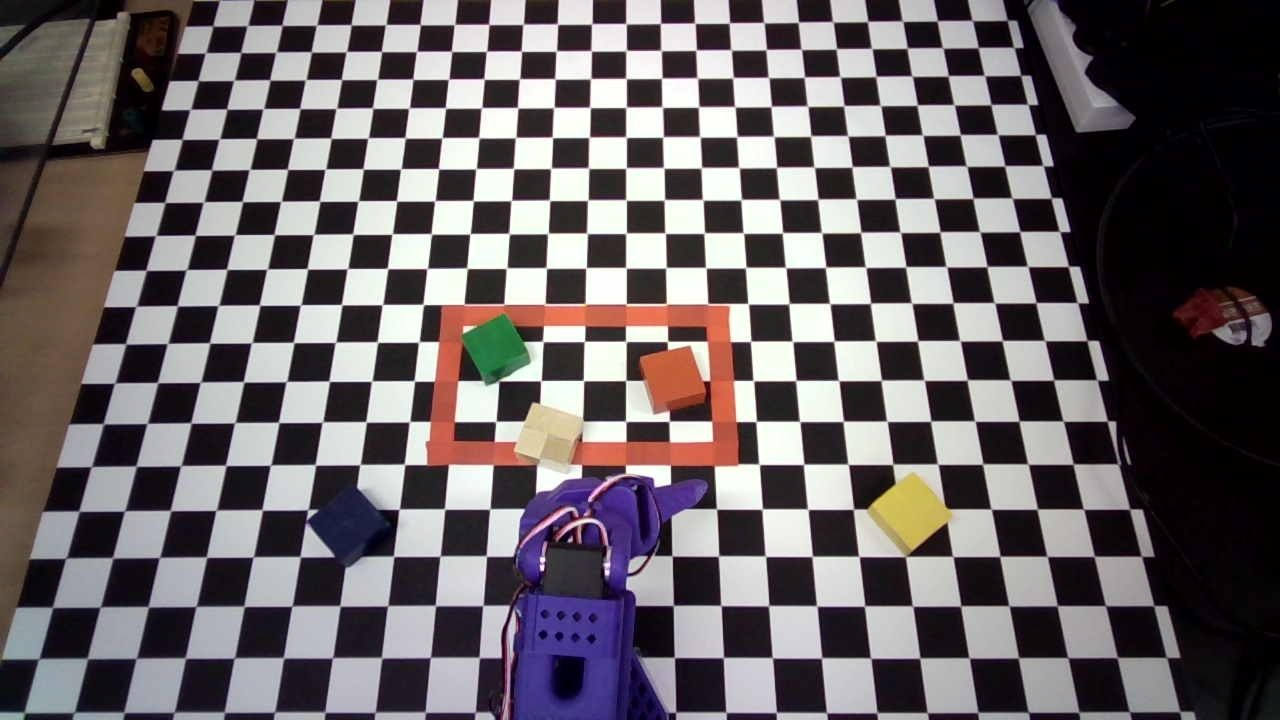
\includegraphics[width=\linewidth]{grasp_before.jpg}
\caption{첫 위치의 실행 전 장면}
\end{subfigure}\hfill
\begin{subfigure}{0.48\linewidth}
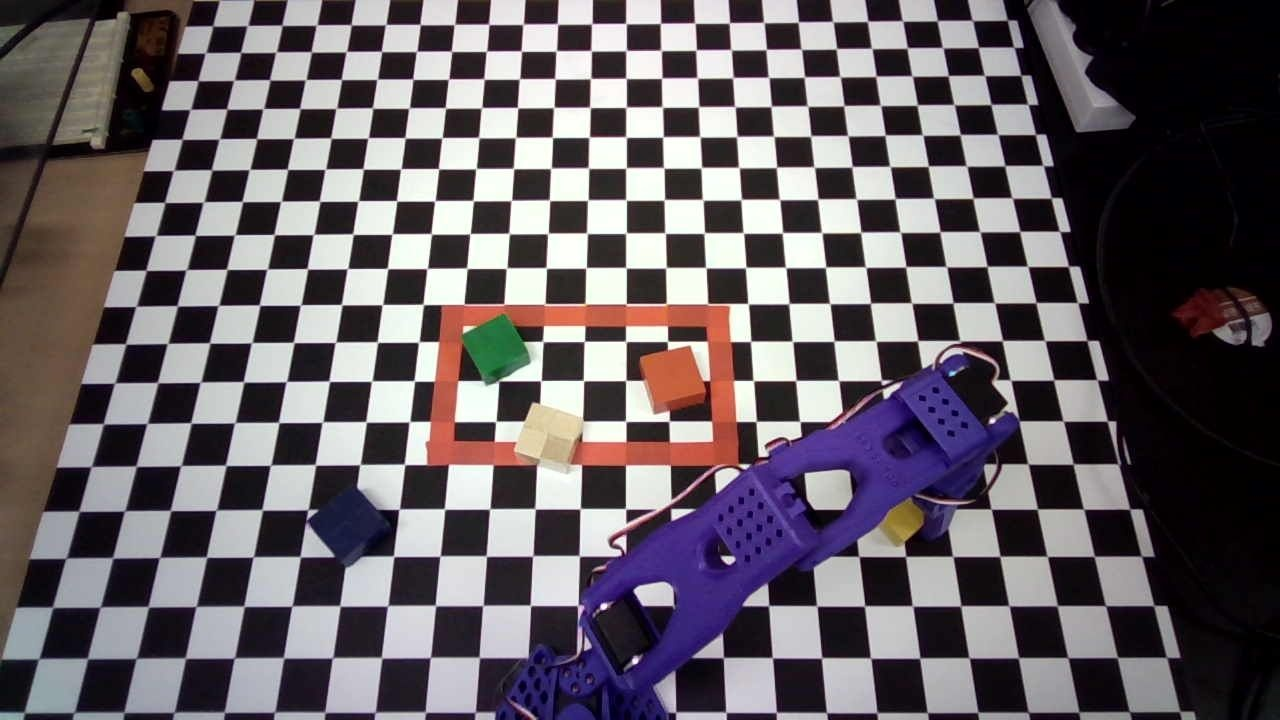
\includegraphics[width=\linewidth]{grasp_lifted.jpg}
\caption{첫 위치의 들어 올린 장면}
\end{subfigure}
\par\medskip
\begin{subfigure}{0.48\linewidth}
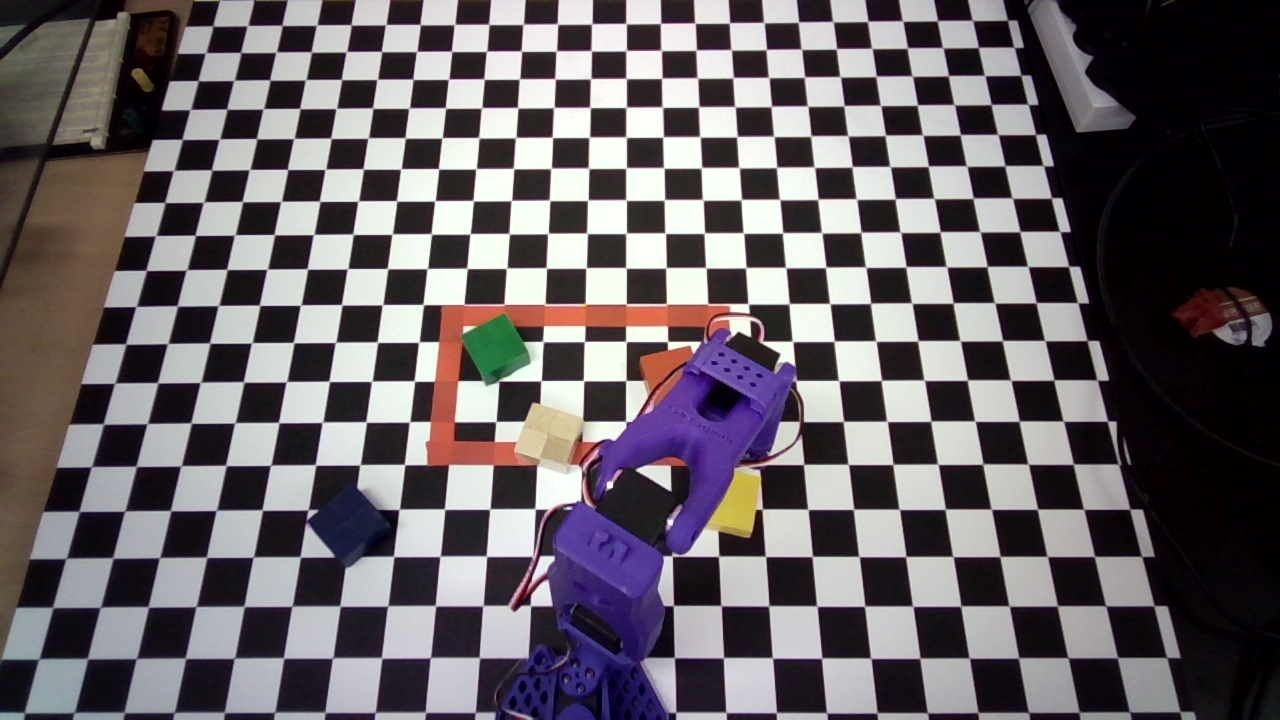
\includegraphics[width=\linewidth]{grasp_inner.jpg}
\caption{안쪽 위치의 닫힘 장면}
\end{subfigure}\hfill
\begin{subfigure}{0.48\linewidth}
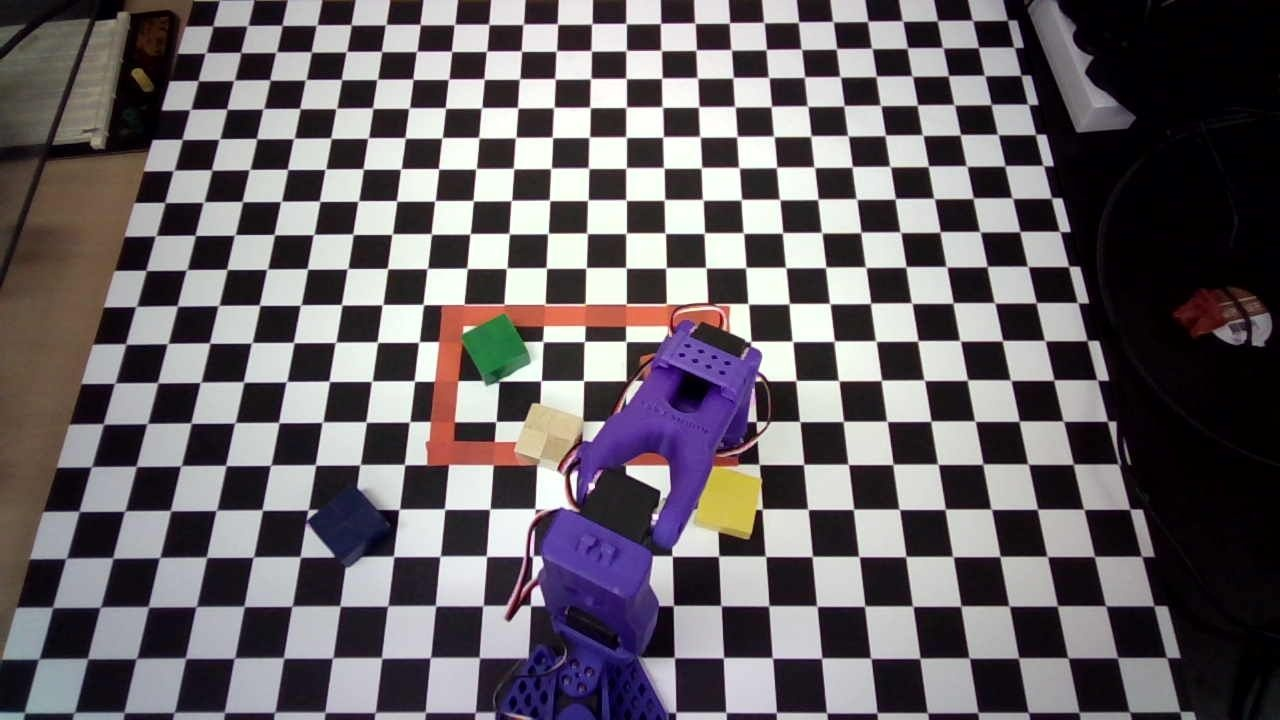
\includegraphics[width=\linewidth]{grasp_retry.jpg}
\caption{보정 재시도의 닫힘 장면}
\end{subfigure}
\caption{노란 블록 시험의 원본 단계 사진. 성공·실패 판정은 사진과 함께 표~\ref{tab:pick-results}의 센서 기록 및 세션 관찰에 근거한다.}
\label{fig:pick-trials}
\end{figure}

실패한 두 시도에서도 FK와 보정된 목표 사이의 거리는 약 1--2\,mm였다. 이는 모델 기준 목표 도달과 실제 파지가 서로 다른 평가라는 점을 보여준다. 특히 목표 좌표 자체에 보정이 적용되어 있으므로 FK--목표 거리가 작다는 사실은 블록의 실제 윗면 중앙에 턱이 정확히 정렬되었다는 의미가 아니다.

첫 위치와 안쪽 위치 사이에는 블록의 위치뿐 아니라 방향도 변화하였다. 따라서 세 시도를 이용하여 위치 효과와 방향 효과를 분리하거나 특정 보정이 성공률을 개선한다고 결론 내릴 수 없다. 이 자료는 독립적으로 구성한 반복 성공률 실험이 아닌, 동작 가능성과 실패 양상을 확인한 진단 사례이다.

\subsection{미션별 달성 범위}
\begin{longtable}{@{}L{0.24\linewidth}L{0.35\linewidth}L{0.31\linewidth}@{}}
\caption{최종 시스템의 구현 및 검증 상태}\label{tab:status}\\
\toprule 항목 & 확인한 내용 & 남은 검증 또는 준비 \\\midrule
\endfirsthead
\toprule 항목 & 확인한 내용 & 남은 검증 또는 준비 \\\midrule
\endhead
고전 CV 인식 & 색·형상·기준점 할당과 작업 영역 필터 구현 & 정답 영상 집합의 검출 정확도·누락률 \\
평면 변환 & 아홉 점의 적합과 LOO 결과 확보 & 품질 기준 미달, 독립 위치 실측 \\
IK·단일 파지 & 실제 노란 블록 파지·들기 및 실패 판정 기록 & 다양한 위치·방향의 반복 결과 \\
1차 배치 & 슬롯 IK와 반복 흐름, 시연 영상 및 제한시간 시험 & 동일 조건의 다섯 블록 완주율·시간 통계 \\
2차 적재 & 적재 전략과 접촉 감지 코드 존재 & 필수 자세 기록, 적재 실행과 5초 유지 \\
관제 도구 & 카메라·검출·FK 관측 경로 구현 & 실제 턱의 영상 위치 보정과 분리 평가 \\
시간 제한 & 180초 외부 제한을 사용한 시험 기록 & 미션 종료·정리 동작의 시간 경계 검증 \\
\bottomrule
\end{longtable}
\FloatBarrier

\section{실패 사례와 검증 한계}
\subsection{실패 단계의 구분}
실패는 검출, 좌표·계획, 파지, 운반·배치, 완료 판정 단계로 나누어 해석하였다. 팔에 의해 블록이 가려지면 검출을 새로 얻지 못할 수 있으며, 실제 세션에서 재시도 계획을 실행하기 전에 관측이 가려져 중단한 사례가 있었다. HOME으로 이동하여 시야를 확보한 뒤 다시 시도한 기록과 구분하여, 계획 단계 중단을 실행된 파지 실패 횟수에 섞지 않는다.

계획 단계에서는 슬롯 보정을 적용한 목표가 IK 게이트를 넘을 수 있다. 이 경우 dry-run의 실패는 실행 전 계획 제한에 해당한다. 파지 단계에서는 관절 목표에 도달했더라도 빈손 닫힘이 발생할 수 있다. 운반 전에는 그리퍼 유지 명령에 따라 부하가 달라질 수 있으며, 9월 8일 보조 시험에서 앞선 종료 처리 후 낮아진 부하를 정상 닫힘 명령으로 회복한 관찰이 남아 있다. 이러한 조건 변화는 단일한 ``좌표 오차''로 합치지 않는다.

완료 판정은 인식 결과에 의존한다. 외부 검출이 없다는 상태에는 모든 블록이 배치된 경우뿐 아니라 작업 영역 필터나 형상 조건에서 물체가 빠진 경우도 포함될 수 있다. 따라서 향후에는 각 색의 실제 배치 위치를 확인하거나, 별도의 검증 영상에서 블록 전체 경계와 영역 포함 여부를 판정하는 방법을 검토할 필요가 있다.

\subsection{소프트웨어 시험과 실기 성능의 구분}
프로젝트 기록에는 구조 정리 후 로컬 환경에서 94개 테스트 통과와 IK 모듈 건너뜀, Orin 환경에서 IK를 포함한 99개 테스트 통과가 남아 있다. 이 수치는 당시 개발 기록이며 이번 보고서 작성 과정에서 실기 시험을 새로 수행한 결과가 아니다. 테스트는 설정 계약, 검출·선택 동작, 카메라 인터페이스, FSM과 계산의 회귀를 확인하는 근거로 사용한다.

단위 테스트에 사용한 모의 로봇이나 합성 영상은 실제 마찰, 관절 유격, 조명 변화와 통신 상태를 모두 재현하지 않는다. 테스트 통과 수를 파지 성공률이나 미션 완주율로 환산하지 않는다. 특히 정리 후 모터 동작을 재검증하지 않은 구간은 코드 검증과 하드웨어 검증을 별도로 표시하였다.

\subsection{추가 평가의 설계}
후속 평가에서는 초기 위치와 방향을 기록한 세트를 만들고, 같은 조건을 반복하여 단일 파지와 전체 미션을 별도로 집계해야 한다. 각 시행에는 실행 코드 버전, 활성 캘리브레이션, 적용한 보정값, 영상 및 상태 전이를 연결한다. 성공률은 성공 횟수를 전체 시행 횟수로 나누어 산출하되, 시간 제한 중단과 계획 거부를 어떤 단위의 실패로 세는지 미리 정한다.

원인 분리를 위한 실험에서는 위치, 방향, 보정 여부, 카메라 상태 중 한 번에 하나만 변경한다. 2차 미션은 필수 자세와 하강 범위의 사전 검토 후 낮은 적재 단계부터 접촉 판정과 해제 후 유지시간을 확인해야 한다. 이 절의 내용은 아직 수행하지 않은 평가 계획이며 현재 성능 결과에 포함하지 않는다.

\section{구축 및 운용 부담 평가}
모방학습에서 CV+IK로의 전환은 필요한 작업의 종류를 바꾸었다. 모방학습 단계에서는 시연 수집·정비, 모델 학습, 추론 환경 구성과 정책 동작 평가가 필요하였다. 최종 경로는 정책 학습을 요구하지 않지만 카메라 고정, 대응점 수집, 색 기준과 형상 임계값 조정, 기구학 보정과 상태별 재시도를 설계해야 한다.

\begin{table}[htbp]
\centering
\caption{개발 경험에 근거한 구축·운용 부담의 정성 비교}\label{tab:cost}
\begin{tabularx}{\linewidth}{@{}L{0.19\linewidth}YY@{}}
\toprule 항목 & 초기 모방학습 경로 & 최종 CV+IK 경로 \\
\midrule
준비 자료 & 시연 에피소드와 학습 설정 & 대응점, 색·형상 설정, 로봇 자세 \\
연산 구성 & 모델 학습·추론과 원격 연결 & 영상 처리와 웨이포인트 IK \\
환경 변경 & 관측 변화에 따른 데이터·정책 재검토 & 마운트 변경 시 재캘리브레이션, 조명 변화 시 검출 재검토 \\
오류 분석 & 정책 출력과 실패 구간, 데이터 분포 검토 & 검출·좌표·IK·센서·상태 단계별 검토 \\
확장 부담 & 새 과제·물체에 대한 데이터와 정책 검증 & 물체 형상·색, 추적·배치 규칙 재설계 \\
확보한 수치 & 중간 단계 112개 에피소드, ACT 집계 29/50 & 아홉 점 적합과 LOO, 개별 실기 관찰 \\
\bottomrule
\end{tabularx}
\end{table}

표~\ref{tab:cost}는 비용을 원화나 인시로 측정한 결과가 아니다. 두 경로에 투입된 실제 작업시간과 하드웨어 사용 비용이 충분히 기록되지 않아 정량 비용 우열을 제시할 수 없다. 다만 CV+IK의 캘리브레이션·규칙 설계 부담을 제외한 채 성공률만 비교하는 설명은 피하고, 구현 방식의 선택에 따라 어떤 부담이 생겼는지를 드러냈다.

\section{산학협력 자문의견에 대한 보완 및 대응}
2026년 8월 3일 삼성중공업 이재민 프로의 서면 자문은 중간보고서의 미션 정의와 후보 구조, 단계별 실패 기록 방식을 긍정적으로 평가하면서 설계 가정과 실제 검증의 구분, 후보 선정 기준 및 전체 구축 비용의 고려를 요구하였다. 본 초안은 자문 항목을 표~\ref{tab:mentor}와 같이 반영하였다.

\begin{longtable}{@{}L{0.22\linewidth}L{0.39\linewidth}L{0.29\linewidth}@{}}
\caption{자문의견에 대한 반영과 남은 한계}\label{tab:mentor}\\
\toprule 자문의견 & 보고서와 구현에 반영한 내용 & 남은 한계 \\\midrule
\endfirsthead
\toprule 자문의견 & 보고서와 구현에 반영한 내용 & 남은 한계 \\\midrule
\endhead
설계·구현·검증 구분 & 1장에 보고 범위를 선언하고 표~\ref{tab:status}에 구현과 실기 확인을 구분. 2차 필수 자세의 미등록 상태도 명시. & 미션별 반복 성능 자료가 부족함. \\
데스크톱 추론 우수성은 가정 & 원격 추론 구축은 과거 수행 내용으로 설명. 최종 실행에서는 정책 추론을 사용하지 않음. & 동일 조건의 장치별 추론 비교 미완료. \\
색상 혼동의 근거 필요 & 빨간 테이프와 색 후보의 문제를 형상·기준점·영역 필터로 다룸. & 오검출·누락의 정답 영상 기반 통계 미확보. \\
ACT--CV/IK 전환 조건 불명확 & 최종 설계를 정책과 규칙의 실행 중 전환이 아닌, 고전 CV+IK 경로로 정리. & 초기 하이브리드의 완전한 실기 비교 미완료. \\
후보 중단·선정 기준 필요 & 제한된 일정, 초기 파지 관찰과 단계별 진단 필요성을 선정 근거로 설명. & 사전에 고정한 기준에 따른 전면 비교는 수행하지 못함. \\
성공률 외 구축·유지 비용 고려 & 표~\ref{tab:cost}에 데이터·학습과 캘리브레이션·규칙·환경 변경 부담을 함께 제시. & 실제 인시·금전 비용의 정량 기록 부족. \\
ACT 반복 횟수 미기록 & 팀 제공 집계를 반영하여 29/50회, 58\%로 구체화하고 평가 단위를 단일 블록 이동으로 명시. & 개별 시행 로그와 조건의 추가 확인 필요. \\
두 미션의 목표 달성 미검증 & 최종 신경망 미사용 경로와 미션별 달성 범위를 설명. 적재 유지 결과는 미검증으로 표시. & 2차 적재 실기와 두 미션의 반복 평가 필요. \\
\bottomrule
\end{longtable}

자문에 대한 대응은 모든 지적 사항의 검증을 완료했다는 의미가 아니다. 구현 경로를 명확히 하고 현재 자료로 말할 수 있는 범위를 정리한 부분과, 추가 실험이 필요한 부분을 함께 제시하였다. 최종 제출 전에는 초안의 추가 확인 항목을 검토하여 새로 확보한 근거만 반영해야 한다.
\FloatBarrier

\chapter{결론 및 향후 연구 방향}
\section{결론}
본 과제는 고전 컴퓨터 비전과 역기구학을 이용한 SO-101 블록 이동 제어를 구현하고 실기로 부분 수행하였다. 적재는 PLACE 전략과 접촉 감지의 구현 단계이며, 타워 자세 등록과 통합 실기 검증이 남아 있다. 인식, 파지 후보 계산, 위치/부하 확인, 재시도와 슬롯 배치를 연결하여 동작 결과에 따라 다음 상태를 결정하는 구조를 구성하였다.

외부 180초 제한의 전체 미션 한 회에서는 파지 후보 14회의 실행 시작, HELD 4회, EMPTY 9회와 판정 전 중단 1회를 기록하였다. 네 번의 슬롯 해제 후 마지막 블록이 남아 미션은 미완료였으며, 해제 수를 인정 블록 수로 환산하지 않았다. 별도 단일 블록 시험에서는 첫 위치의 파지와 운반에 성공했지만 안쪽 위치의 기본 시도와 보정 재시도는 빈손으로 판정되었다. 최종 CV+IK의 동일 조건 반복 성공률과 ACT 대비 성능 차이는 측정하지 못하였다.

실행 로그는 노란 블록의 후보 재시도와 빨간 블록의 재선택 후 파지 판정 회복을 보여준다. 반면 빨간 블록의 첫 PICK에 51.5초가 소요되어 재시도의 시간 비용도 확인하였다. 좌표 정합은 RMS 8.18\,mm, 최대 LOO 26.64\,mm로 개발 목표에 미달하였다. 본 연구의 주요 기여는 기존 라이브러리의 영상 처리와 기구학 기능을 과제에 맞는 선택, 계획, 검증 및 복구 흐름으로 통합하고, 실패 단계를 실행 기록으로 분석한 데 있다. 요구된 미션의 안정적인 완수를 입증하려면 다음의 검증과 개선이 필요하다.

\section{향후 연구 방향}
\subsection{동일 조건 반복 평가와 시간 예산 개선}
우선 한 초기 배치를 사진으로 고정하고 코드, 실행 설정과 캘리브레이션을 유지한 상태에서 전체 미션을 3회 반복할 계획이다. 각 시행에 대해 사람이 판정한 인정 블록 수, 시스템 완료 상태, 제한시간 종료와 실제 정리 동작 시간을 따로 기록한다. 파지 영상과 센서 판정을 연결하고 첫 후보, PICK 내부 재시도 및 대상 재선택을 구분한다. 이 소규모 시험은 고정 배치의 반복성 평가이며, 무작위 배치의 일반화 평가는 별도로 수행한다.

현재의 실패 기록을 바탕으로 후보별 시간 상한과 다음 블록으로의 전환 시점을 우선 검토한다. 성능 측정 중에는 설정을 변경하지 않고, 이후 같은 배치에서 재시도 정책을 변경한 결과를 비교한다. 실제 턱과 블록의 상대 위치 측정, 파지 직전 영상 보정, 검출 누락과 물리적인 완료 조건의 차이도 후속 개선 대상으로 둔다.

\subsection{적재 높이별 동작 개선과 실기 평가}
\label{sec:stack-extension}
적재는 타워 접근과 하강 자세를 등록한 뒤 높이별 도달성, 관절 한계와 그리퍼 개방 공간부터 확인한다. 접촉 감지와 되돌림 후 해제가 아래 블록을 밀거나 타워를 흔드는지 2단과 3단에서 평가하고, 이후 다섯 블록과 5초 유지 조건으로 확대한다. 각 단계의 시도 횟수, 실패 단계와 유지시간을 기록하며 현재는 낮은 단수의 실기 성공도 확인되지 않았다.

평면 변환은 블록 한 개의 윗면을 기준으로 하므로 타워가 높아졌을 때 같은 변환을 그대로 적용할 수 없다. 초기에는 고정한 타워 위치와 기록 자세를 사용하고, 높이 변화에 따른 관측 오차와 적재물 재선택 문제를 별도로 평가한다.

\subsection{규칙 기반 실행의 학습 데이터 활용}
\label{sec:dataset-extension}
미션의 반복 수행과 결과 판정이 안정화되면 CV+IK 실행 중 영상, 관절 상태와 전달 명령을 같은 시간 기준으로 기록하는 확장을 검토한다. 초기에는 사람이 블록을 재배치하고, 단일 블록 선택부터 배치 후 재관측까지를 한 에피소드로 구성한다. 내부 재시도, 실패, 시간 초과와 사람의 확인 결과를 함께 저장하며, 현재의 사진 및 텍스트 기록에 동기화와 에피소드 구성 기능을 추가해야 한다.

저장 형식은 사용할 LeRobot 버전과 호환되도록 선택한다\cite{lerobot-dataset}. 모방학습이나 SmolVLA에 활용하려면 관측과 행동 표현, 작업 지시 및 센서 라벨의 신뢰도를 확인해야 한다\cite{smolvla}. 강화학습용으로 확장할 때에는 다음 관측, 보상과 종료 조건도 정의하고, 파지 라벨을 전체 배치 성공의 보상으로 그대로 대체하지 않는다. 유효 에피소드 수, 기록 누락과 사람의 작업시간으로 수집 방식을 평가하며, 데이터 수집 자동화와 학습 성능 개선은 현재 실증한 성과에 포함하지 않는다.
\FloatBarrier

\clearpage
\begingroup
\raggedright
\bibliographystyle{unsrt}
\bibliography{references}
\endgroup
\end{document}
